\section{Solução Implementada}

    O aplicativo Encontre na UFMS foi desenvolvido com o intuito de facilitar a navegação pelo campus da UFMS em Campo Grande, permitindo que usuários encontrem e localizem pontos de interesse dentro do campus, estes sendo cadastrados por outros usuários, possibilitando que locais que não estão presentes em outros aplicativos de localização sejam documentados e compartilhados com a comunidade acadêmica. Os usuários também terão poder de avaliar os locais cadastrados, podendo assim, ajudar outros usuários a escolherem o melhor local para suas necessidades.

\subsection{Análise Crítica e contribuição do Encontre na UFMS}
    Para podermos analisar o diferencial do aplicativo Encontre na UFMS podemos compará-lo com os aplicativos Google Maps e Localização UFMS. O Google Maps é um aplicativo de geolocalização muito utilizado no mundo todo, porém, ele não é focado em um local específico, como o campus da UFMS, e sim em todo o mundo, sendo assim ele não possui registrado diversos locais de menor escala mas que podem ser de grande importância para algum visitante ou alunos. Já o Localização UFMS é um aplicativo web que disponibiliza um mapa interativo da UFMS que possui mais de 2900 pontos de interesse registrados, porém, ele não possui alguns pontos de interesse que podem ser de grande importância para a comunidade acadêmica, como por exemplo, o Restaurante Universitário e também não informa ao usuário como chegar até o local desejado já que ele é focado em apenas mostrar informações sobre um certo local, ele também não tem fotos de todos os locais e não é colaborativo uma vez que apenas a administração da UFMS pode adicionar novos locais.

\subsection{Comparação entre o Encontre na UFMS e outros aplicativos}
\begin{table}[h]
    \begin{tabularx}{\textwidth}{|X|X|X|X|}
        \hline
        \textbf{Características} & \textbf{Google Maps} & \textbf{Localização UFMS} & \textbf{Encontre na UFMS} \\ \hline
        \textbf{Objetivo Principal} & Geolocalização global & Mapa interativo da UFMS & Navegação pelo campus da UFMS \\ \hline
        \textbf{Público-Alvo} & Usuários em geral & Comunidade acadêmica da UFMS & Comunidade acadêmica da UFMS \\ \hline
        \textbf{Principais Funcionalidades} & Busca de locais, rotas, informações de contato, horários de funcionamento & Busca de locais no campus, informações sobre pontos de interesse & Busca de locais, rotas, cadastro colaborativo de locais, avaliações de locais \\ \hline
    \end{tabularx}
    \caption{Comparação entre aplicativos de localização}
    \footnotesize  \centering{\textbf{Fonte: Autor original}}
    \label{tab:comparacao-aplicativos}
\end{table}

\subsection{Implementação}

    O desenvolvimento do aplicativo Encontre na UFMS foi dividido em duas partes principais: o backend e o frontend. Trataremos a seguir de cada uma dessas partes, detalhando as tecnologias utilizadas e as funcionalidades implementadas.

\subsubsection{Frontend}

    O frontend foi desenvolvido utilizando o framework Flutter, que permite o desenvolvimento de aplicativos móveis para Android e iOS a partir de um único código fonte. O Flutter é uma ferramenta moderna e de fácil utilização, que permite a criação de interfaces de usuário atraentes e responsivas.

    O código foi desenvolvido com base na \textit{Clean Architecture}, que é um padrão de arquitetura de software que visa separar as responsabilidades do código em camadas bem definidas, facilitando a manutenção e a evolução do sistema. A arquitetura do aplicativo foi dividida em três camadas principais: a camada de apresentação, a camada de domínio e a camada de dados. A camada de apresentação é responsável por exibir os dados para o usuário e capturar as interações do usuário com o sistema. A camada de domínio contém as regras de negócio do sistema, enquanto a camada de dados é responsável por acessar os dados do sistema, seja de um banco de dados local ou de uma API remota.

    \begin{figure}[h]
        \centering
        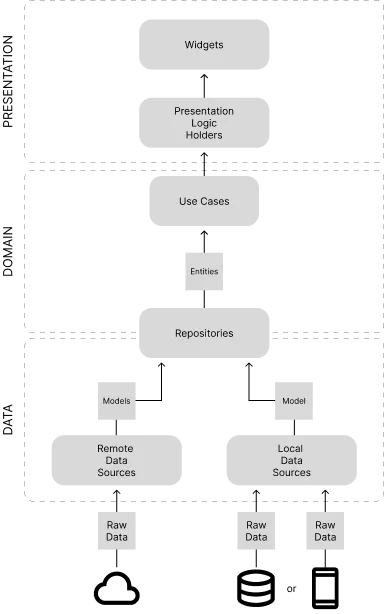
\includegraphics[width=44mm,height=80mm]{imagens/cleanarch.png}
        \caption{\scriptsize Clean Architecture}
        \footnotesize  \centering{\textbf{Fonte: X}}
        \label{fig:clean-architecture}
    \end{figure}

    \FloatBarrier

    Embora o Flutter seja capaz de gerar aplicativos nativos para Android e iOS, o aplicativo Encontre na UFMS foi desenvolvido apenas para Android, visto que a Apple, dona do sistema operacional iOS, restringe o desenvolvimento para seu sistema caso o desenvolvedor não possua um dispositivo da marca. Mas, em teoria, o aplicativo poderia ser facilmente adaptado para iOS, bastando apenas compilar o código fonte em um ambiente de desenvolvimento da Apple.

\subsubsection{Backend}

    O backend foi desenvolvido utilizando o framework Fastify, a fim de garantir excelente desempenho mesmo com um grande volume de requisições, permitindo escalabilidade sem perder a segurança. Foi programado utilizando o Node.js, uma ferramenta que permite a execução de código JavaScript em um ambiente fora do navegador, com excelente desempenho e confiabilidade. 
    
    Durante o desenvolvimento, foi utilizado a linguagem de programação Typescript para tipagem de variáveis, classes e objetos, evitando eventuais erros que poderiam ser causados por incompatibilidade de tipos. Para a execução do código utilizando o Node.js, foi utilizado uma ferramenta do TypeScript para transpilação do código-fonte em JavaScript.

    O código foi desenvolvido utilizando o padrão de software MVC ou Model-View-Controller, sendo em português: Modelo-Visão-Controlador. As três camadas se entrelaçam entre si, onde o Controlador recebe as requisições do usuário e as envia para o Modelo, que manipula os dados e faz a conexão com o banco de dados, após, é retornado para o Controlador que envia para a Visão, que exibe as informações ao usuário. Para a comunicação entre o backend e o frontend, foi utilizado uma API REST.

\subsection{Testes e Execução}

    O aplicativo Encontre na UFMS foi testado em diversos dispositivos Android, a fim de garantir a compatibilidade e o bom funcionamento em diferentes tamanhos de tela e versões do sistema operacional. Foi utilizado o emulador do Android Studio para testar o aplicativo no Pixel 6a na API 33 do Android mas foi principalmente testado em dispositivos físicos, como o Galaxy S21 fe, pela facilidade de uso e para poder verificar a usabilidade real do aplicativo em todo momento.

\subsubsection{Diagrama de Navegação}

    O diagrama de navegação do aplicativo apresentado na Figura 2 demonstra os fluxos básicos de navegação que o usuário pode experenciar
    durante o uso do mesmo, vale destacar que algumas telas como Perfil e Criação só são acessíveis caso o usuário esteja logado.

    \begin{figure}[h]
        \centering
        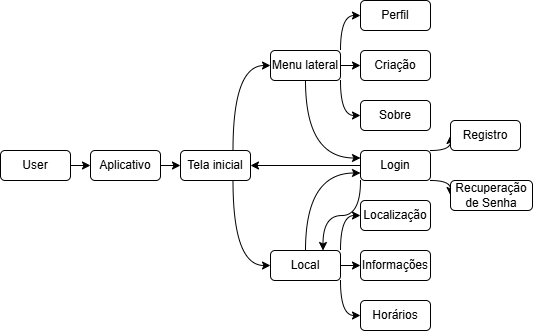
\includegraphics[width=120mm,height=70mm]{imagens/navegacao.png}
        \caption{\scriptsize Diagrama de Navegação}
        \footnotesize  \centering{\textbf{Fonte: Autor original}}
        \label{fig:diagrama-navegacao}
    \end{figure}

    \FloatBarrier

\subsubsection{Tela 1: Listagem de Locais}

    A tela de listagem de locais é a tela inicial do aplicativo, a primeira e principal tela apresentada para o usuário. Nela, o usuário pode visualizar todos os locais cadastrados no aplicativo, podendo filtrar os locais por categoria e buscar locais através de um campo de pesquisa por texto. 
    
    Cada local é representado por um segmento contendo a foto, o nome, o endereço, a categoria, se o local está provavelmente fechado naquele horário e um indicador que mostra se o local está marcado como favorito ou não. Cada segmento é clicável, redirecionando o usuário para a tela de detalhes do local. O usuário pode também clicar no indicador de favorito para marcar ou desmarcar o local como favorito caso ele esteja logado, caso não esteja o usuário é redirecionando para a tela de Login que será abordada mais a frente. A listagem de locais é paginada, exibindo 10 locais por vez, uma nova requisição é feita toda vez que o usuário chega ao final da lista, carregando carregando a próxima página caso haja uma.

    Na parte superior da tela há uma seção com um botão, que abre o menu lateral, e um campo de texto para pesquisa. Logo abaixo há um filtro de categorias, uma série de botões que podem ser arrastados horizontalmente, permitindo que o usuário filtre os locais por uma ou mais categorias, de acordo com suas necessidades. Na busca por texto foi aplicado um \textit{debounce} de 1s para evitar que a busca seja feita a cada caractere digitado, o que poderia causar um consumo excessivo de recursos da API. 

    \begin{figure}[h]
        \centering
        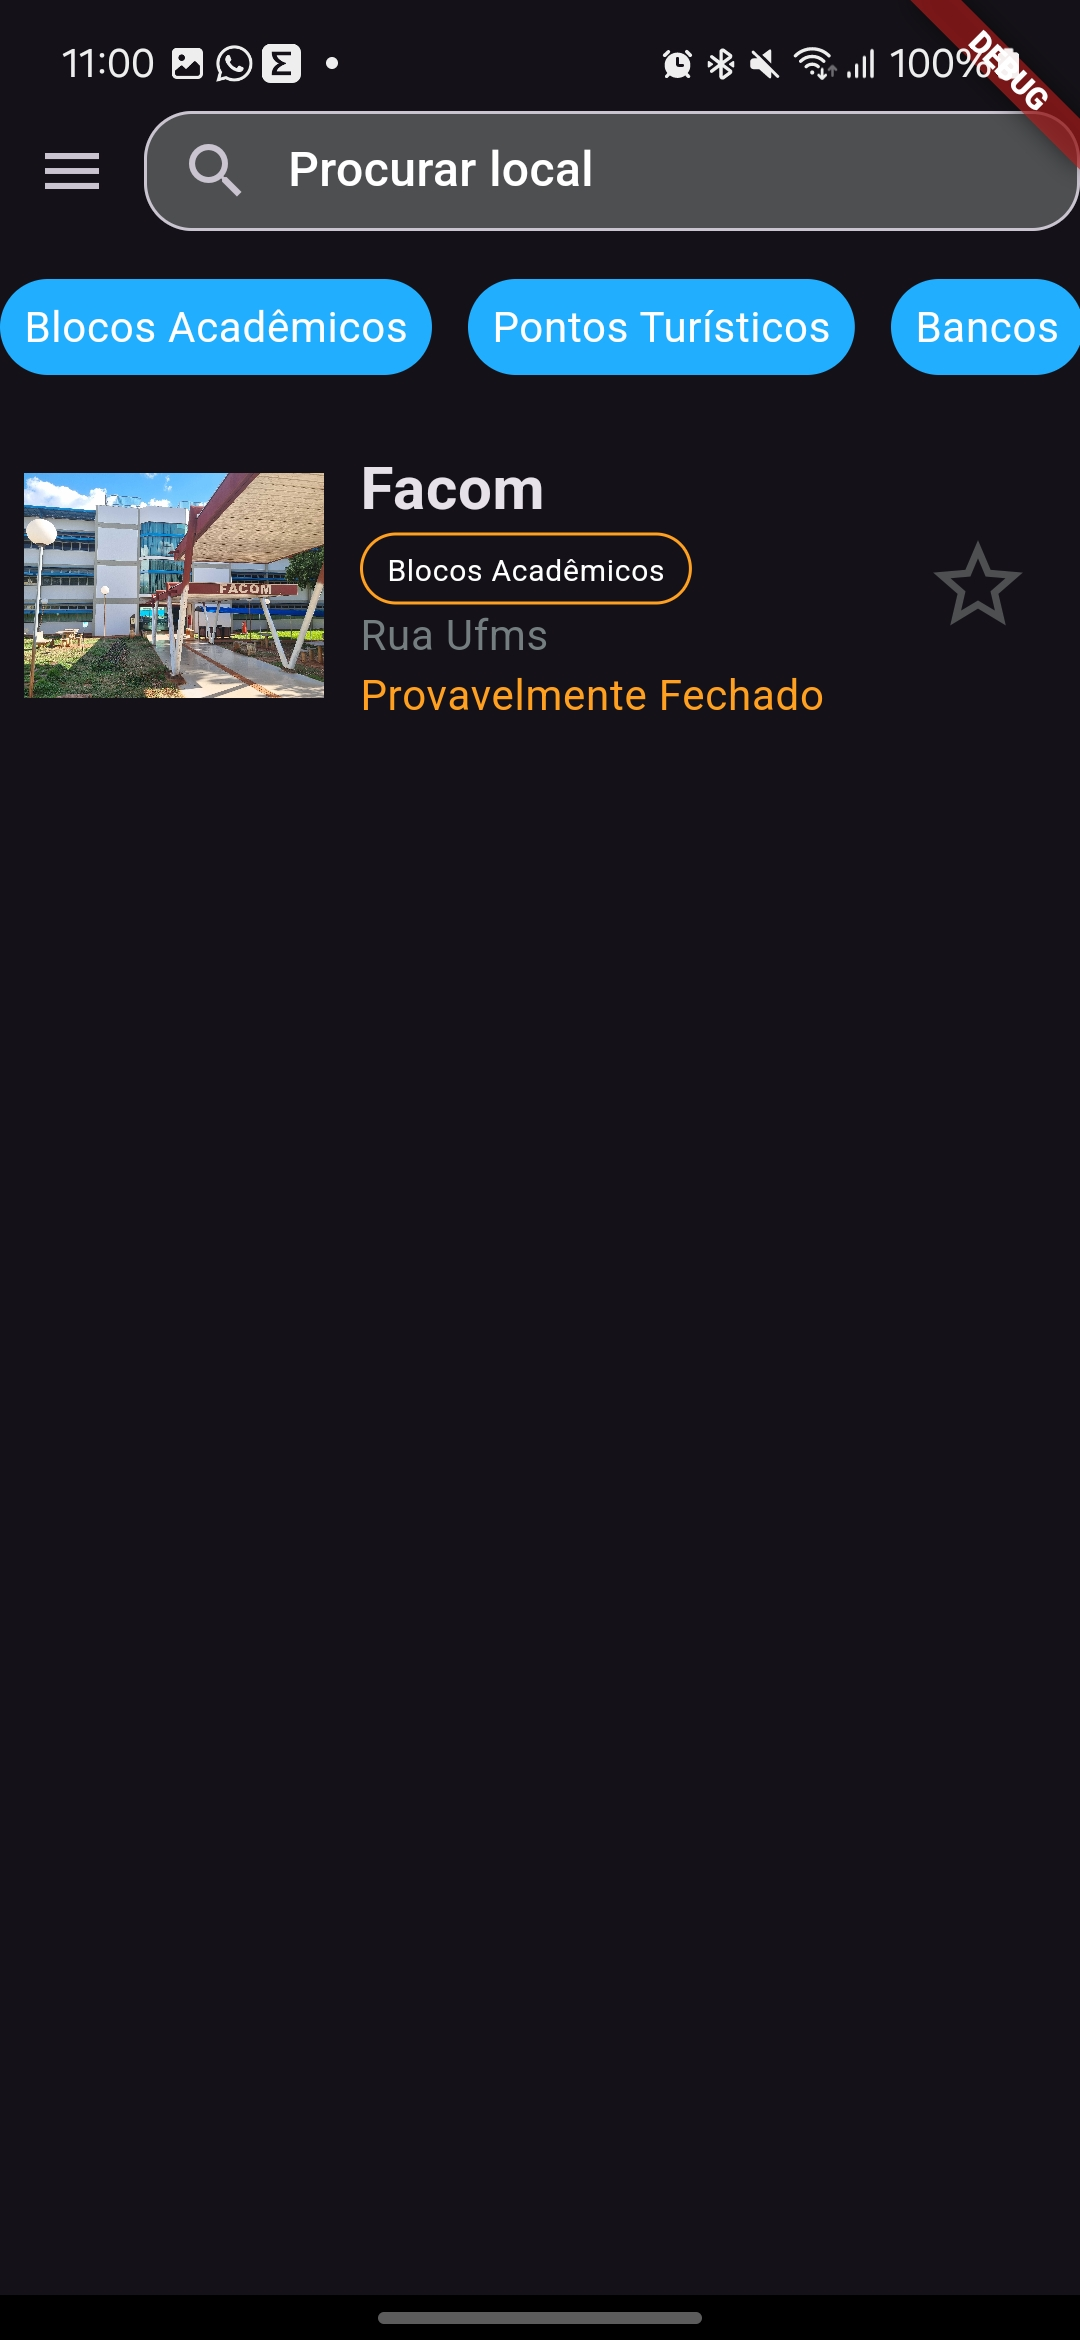
\includegraphics[width=44mm,height=80mm]{imagens/inicial.jpg}
        \caption{\scriptsize Tela 1: Listagem de Locais}
        \footnotesize  \centering{\textbf{Fonte: Autor original}}
        \label{fig:tela1}
    \end{figure}

    \FloatBarrier

\subsubsection{Tela 2: Local}

    A tela de local é onde todos os detalhes do local selecionado pelo usuário na tela de listagem são apresentados. Nela, o usuário pode visualizar uma ou mais fotos do local, o nome, um indicador que é mostrado caso o local tenha opções de acessibilidade e a avaliação média do local, que é a média das avaliações por outros usuários. Além disso existem 3 abas que o usuário pode navegar sem sair da tela. A aba de localização é a aba inicial e mostra o endereço do local, um mapa com a localização do local indicada e uma seção para o usuário dar sua própria avaliação do local, caso esteja logado. A aba de informações exibe alguns detalhes do local como observações e telefone de contato. Por fim, a aba de Horários exibe os horários de funcionamento do local, caso estejam cadastrados.

    \begin{figure}[h]
        \centering
        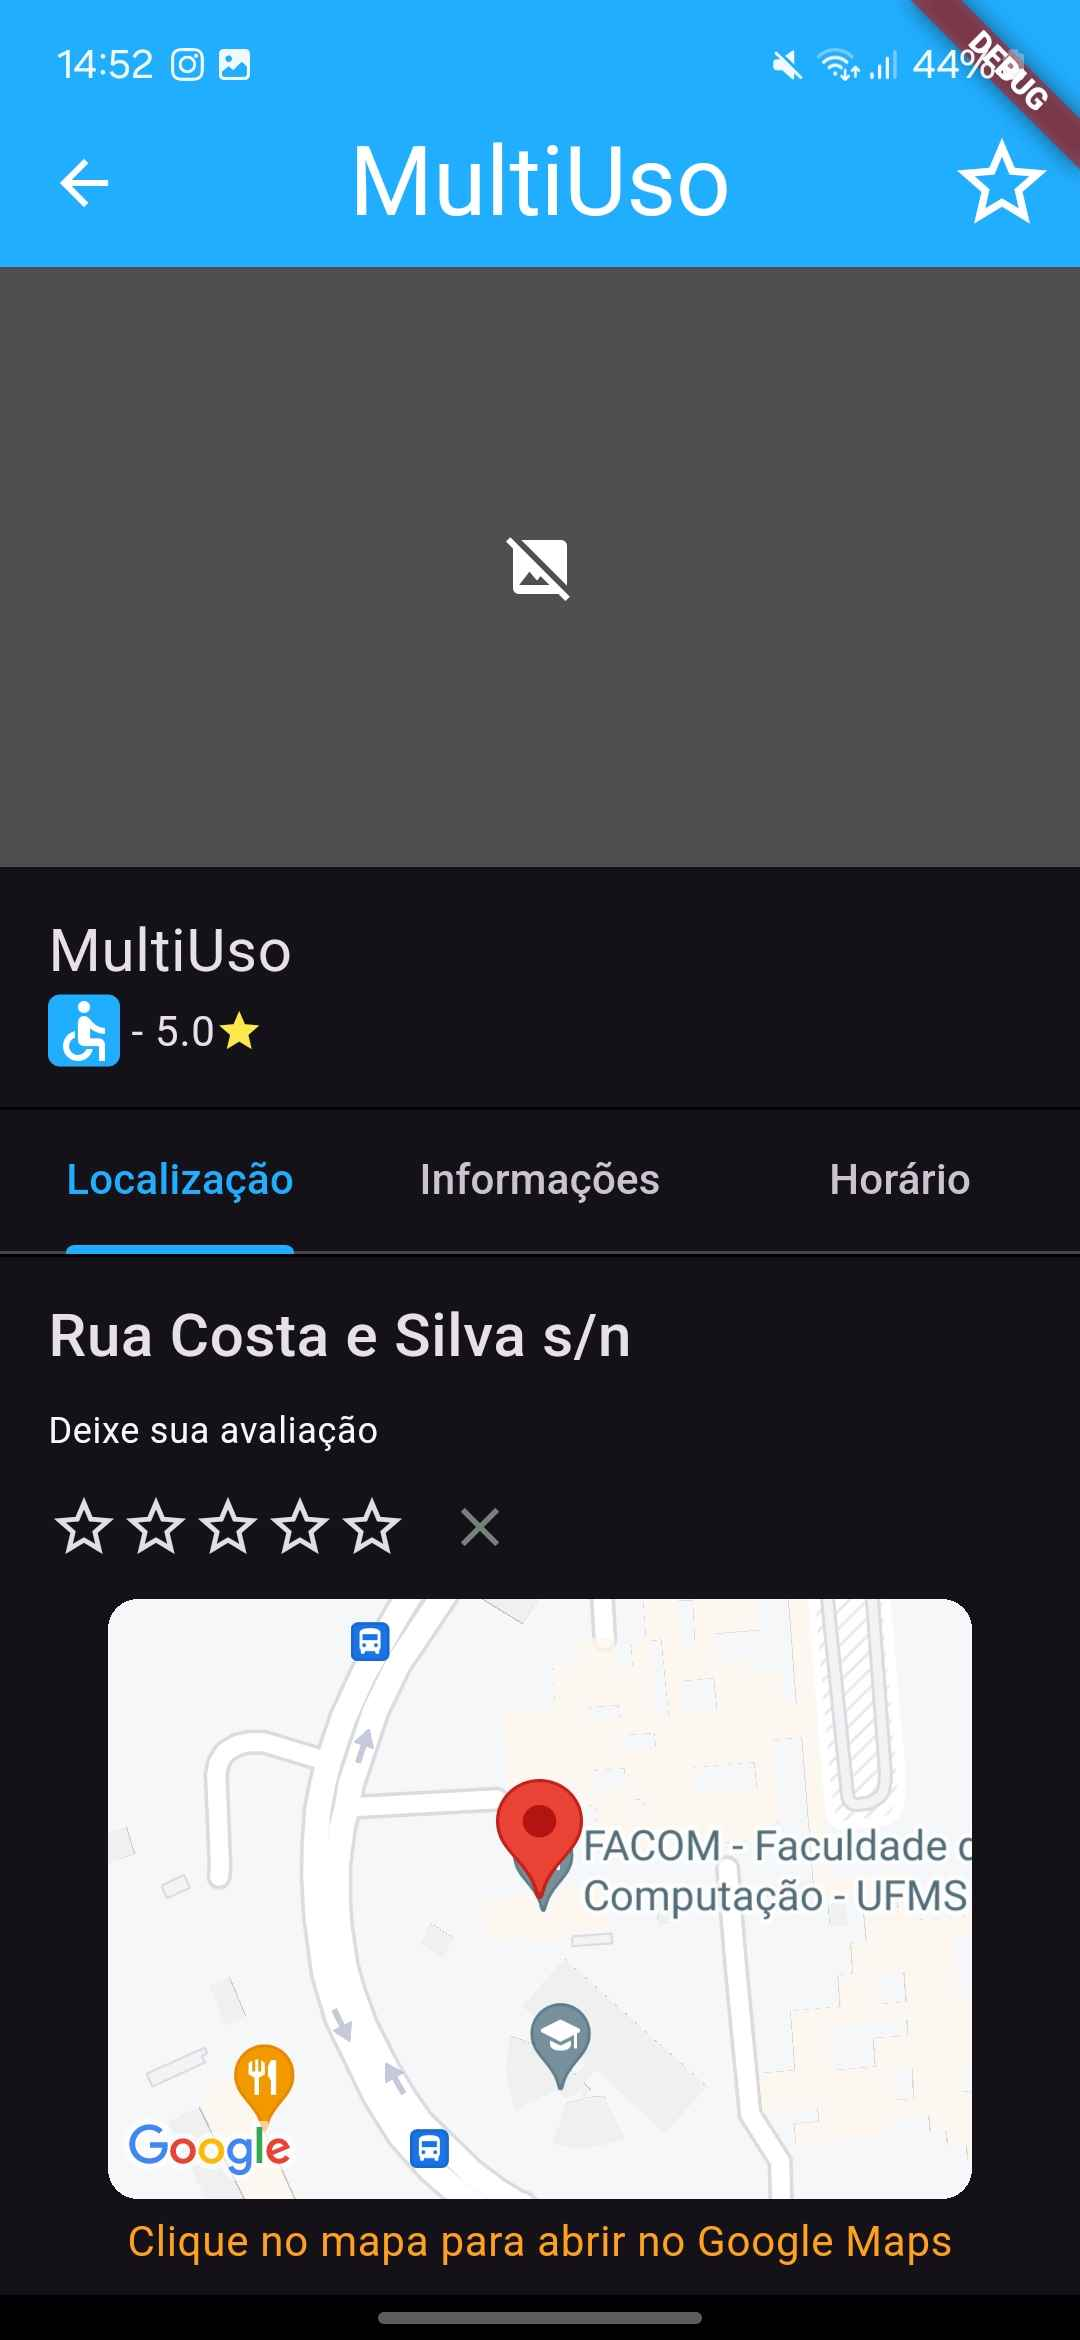
\includegraphics[width=44mm,height=80mm]{imagens/local.jpg}
        \caption{\scriptsize Tela 2: Local}
        \footnotesize  \centering{\textbf{Fonte: Autor original}}
        \label{fig:tela2}
    \end{figure}

    \begin{figure}
        \centering
        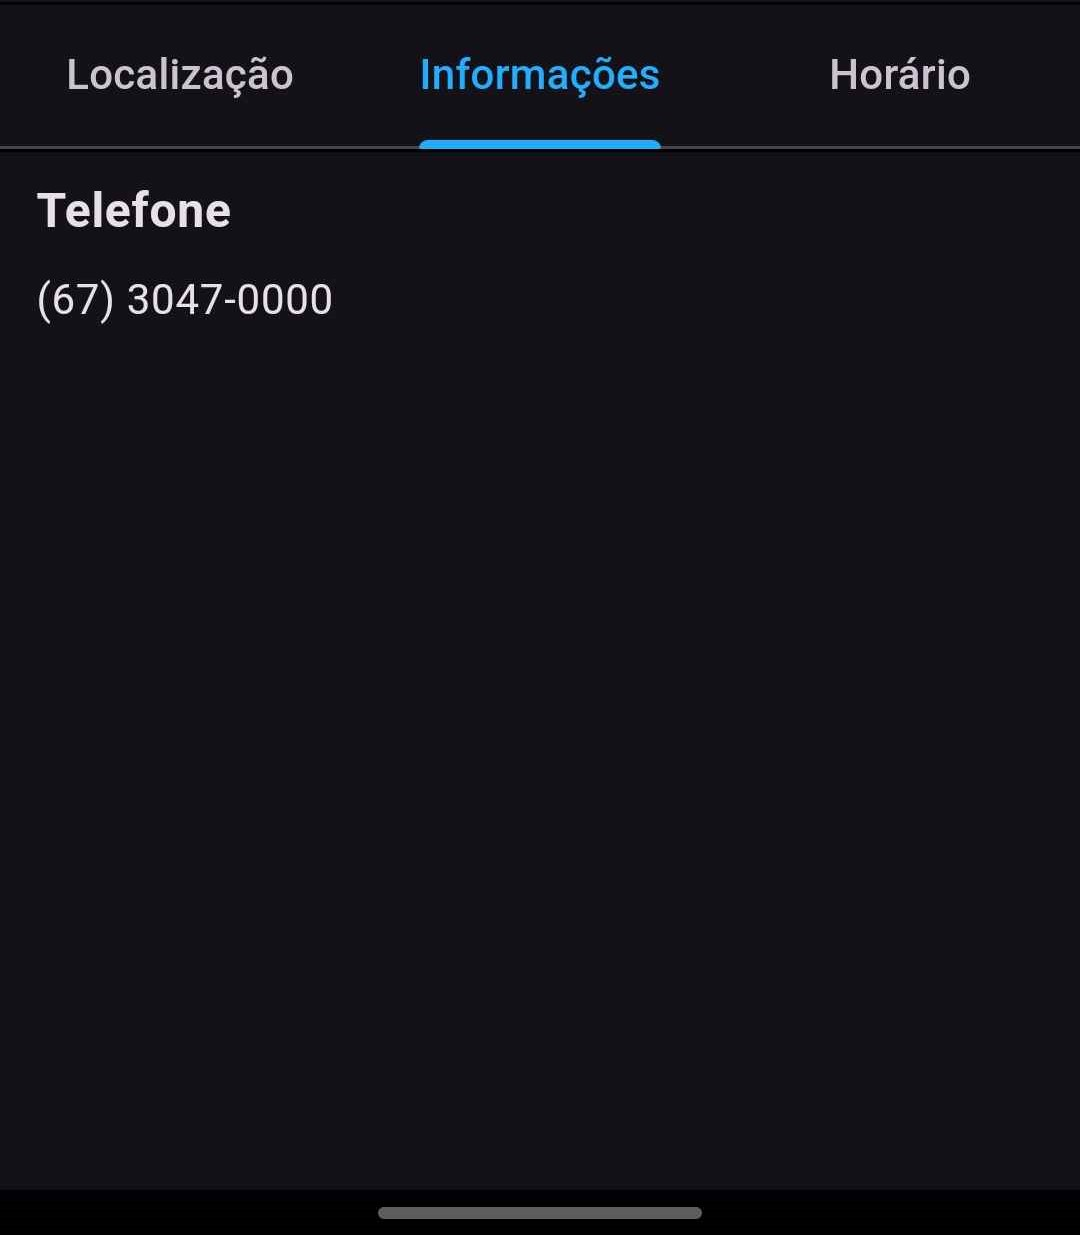
\includegraphics[width=44mm,height=48mm]{imagens/info.jpg}
        \hspace{10mm}
        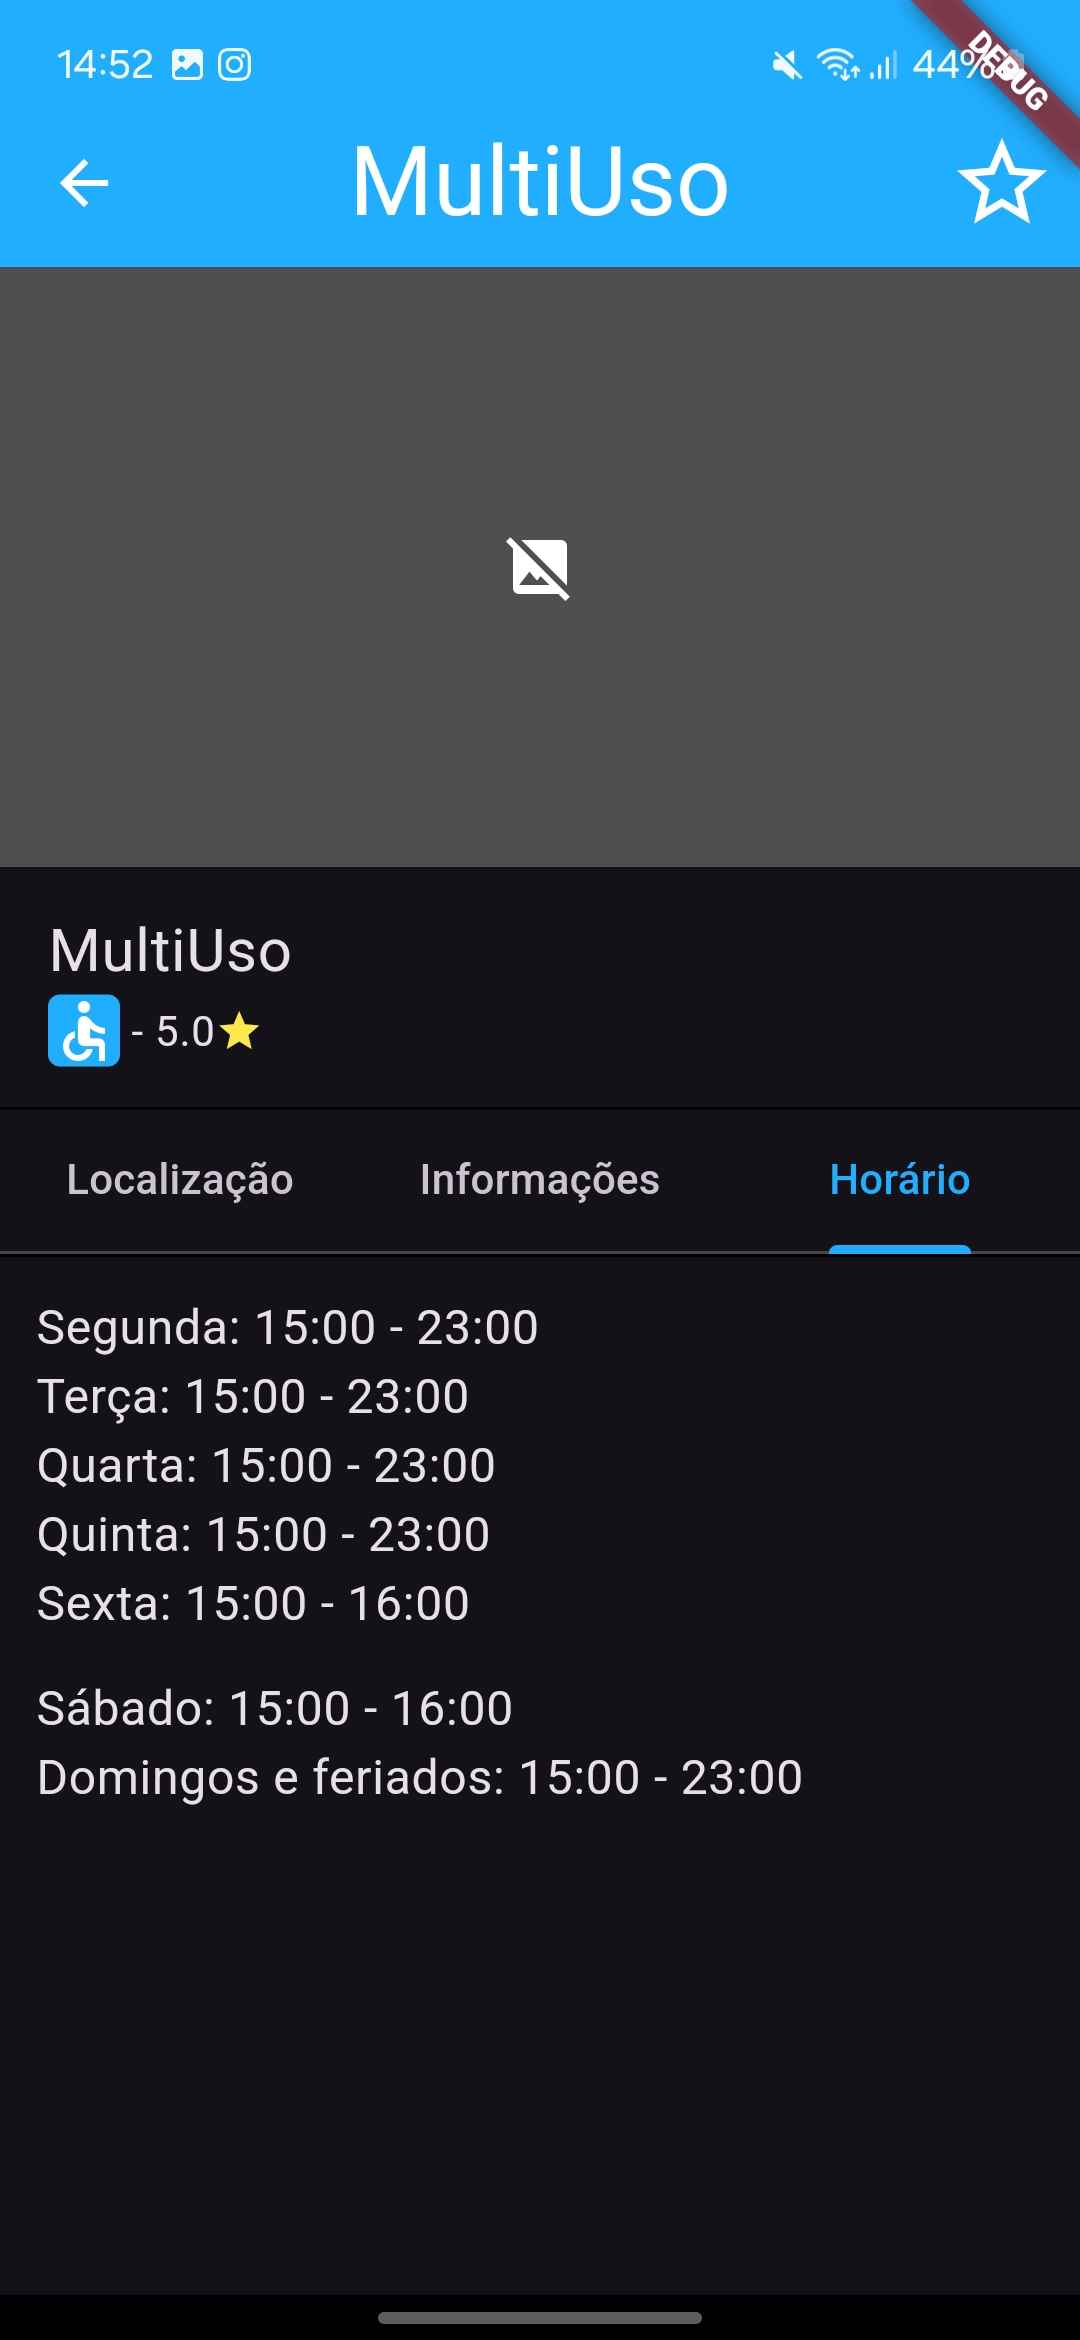
\includegraphics[width=44mm,height=48mm]{imagens/horario.jpg}
        \caption{\scriptsize Abas: Informações e Horários}
        \footnotesize  \centering{\textbf{Fonte: Autor original}}
        \label{fig:tela2-abas}
    \end{figure}

    \FloatBarrier

\subsubsection{Tela 3: Menu Lateral}

    O menu lateral é acessível através de um botão na parte superior da tela de listagem de locais. Ele é composto por uma série de botões que redirecionam o usuário para diferentes telas do aplicativo. O menu lateral é uma forma de organizar as funcionalidades do aplicativo de forma intuitiva e acessível, permitindo que o usuário navegue facilmente entre as diferentes telas do aplicativo.

    Essa tela muda de acordo com o estado de autenticação do usuário, caso ele esteja logado, aparecerá o nome do usuário logo abaixo o nome do aplicativo e os botões de Perfil e Criação assim como um botão de Sair, caso contrário, todas essas informações são omitidas e apenas o botão de Sobre é exibido, e no lugar do botão de Sair é exibido o botão de Login. Abaixo as duas figuras exemplificam ambos os estados.

    \begin{figure}[h]
        \centering
        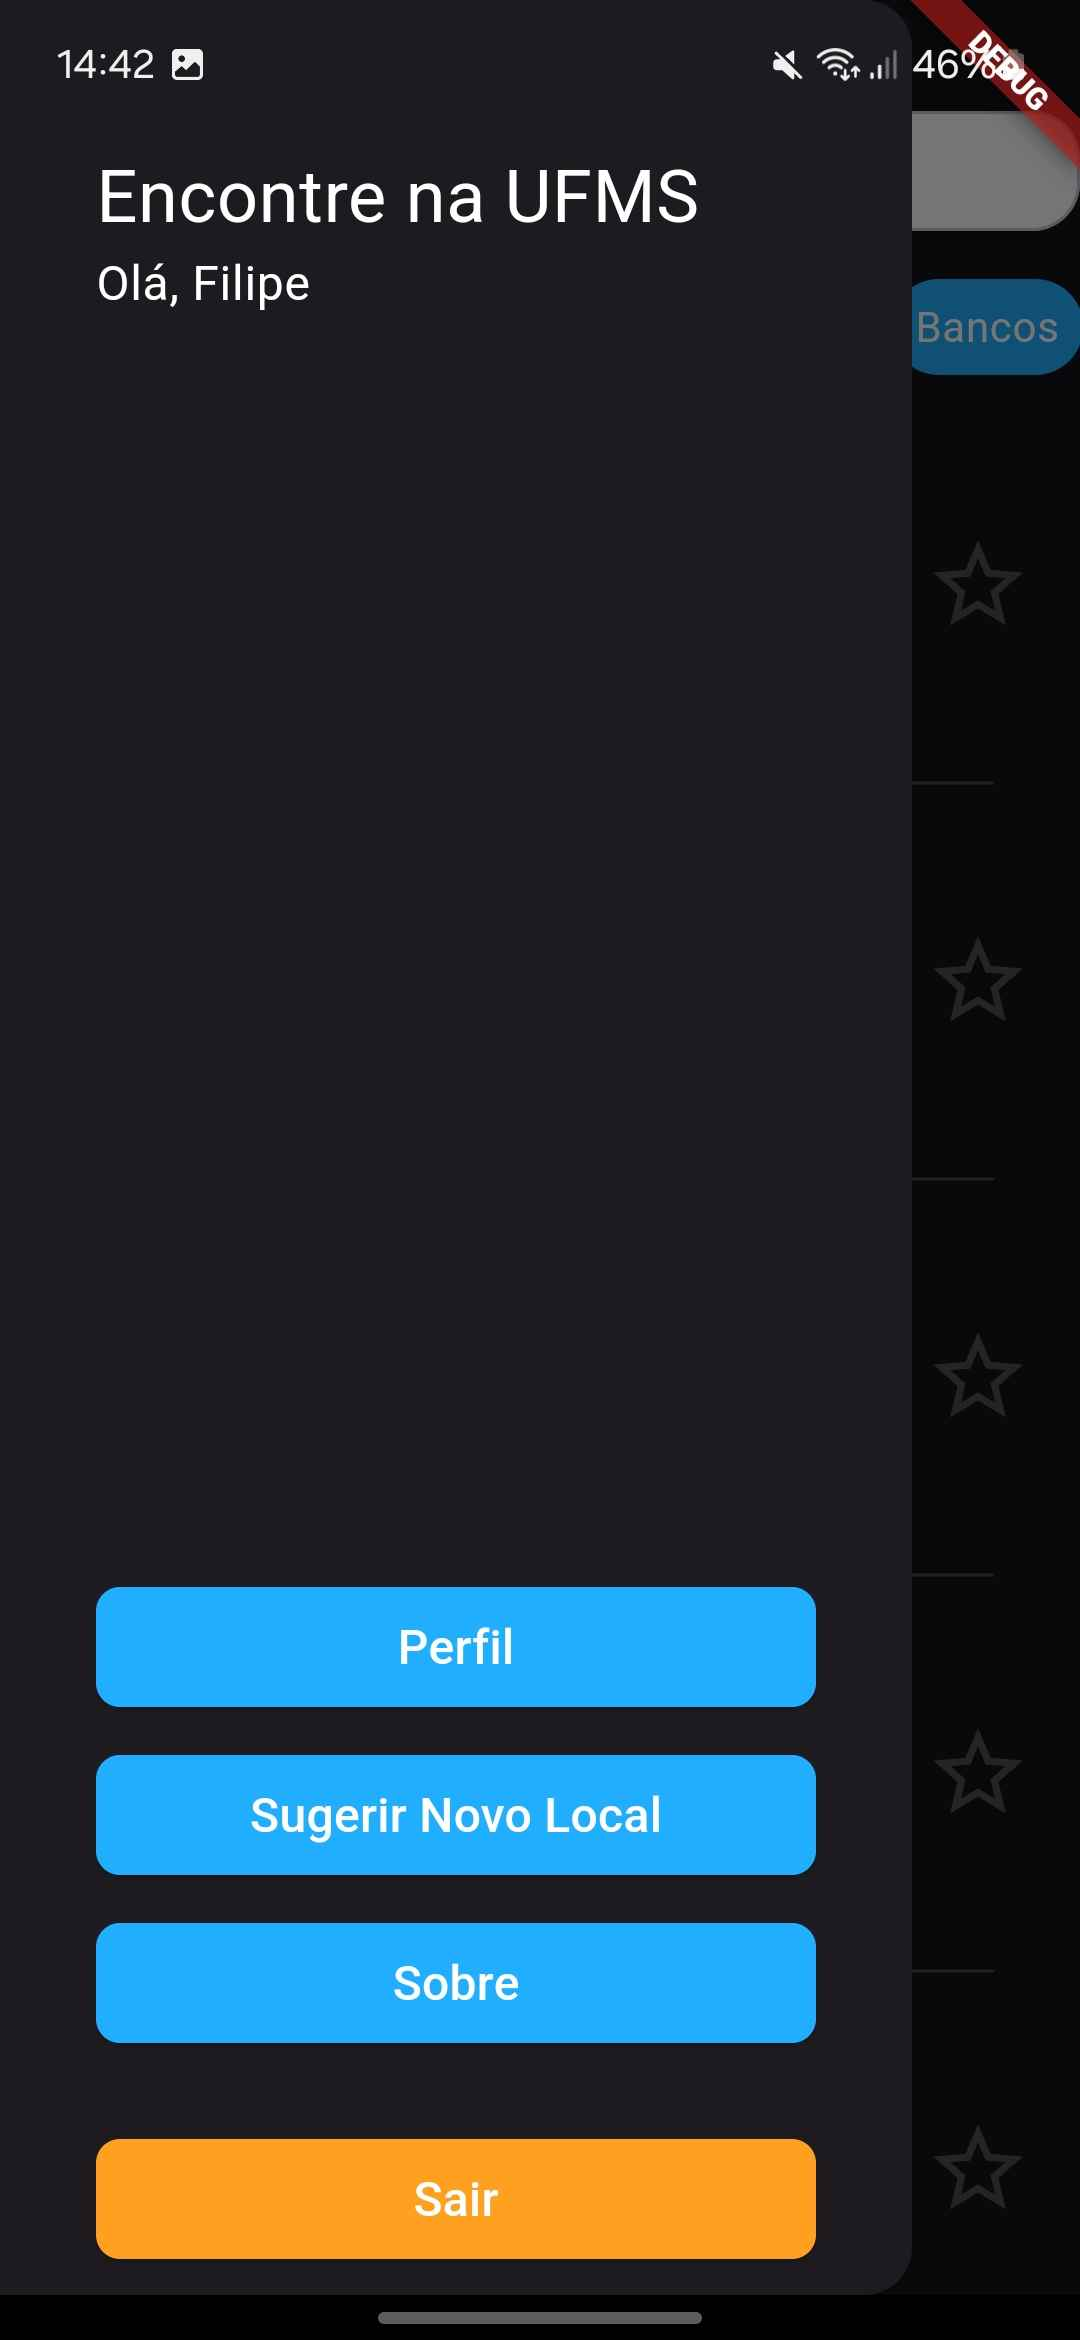
\includegraphics[width=44mm,height=80mm]{imagens/menu-lateral-logado.jpg}
        \hspace{10mm}
        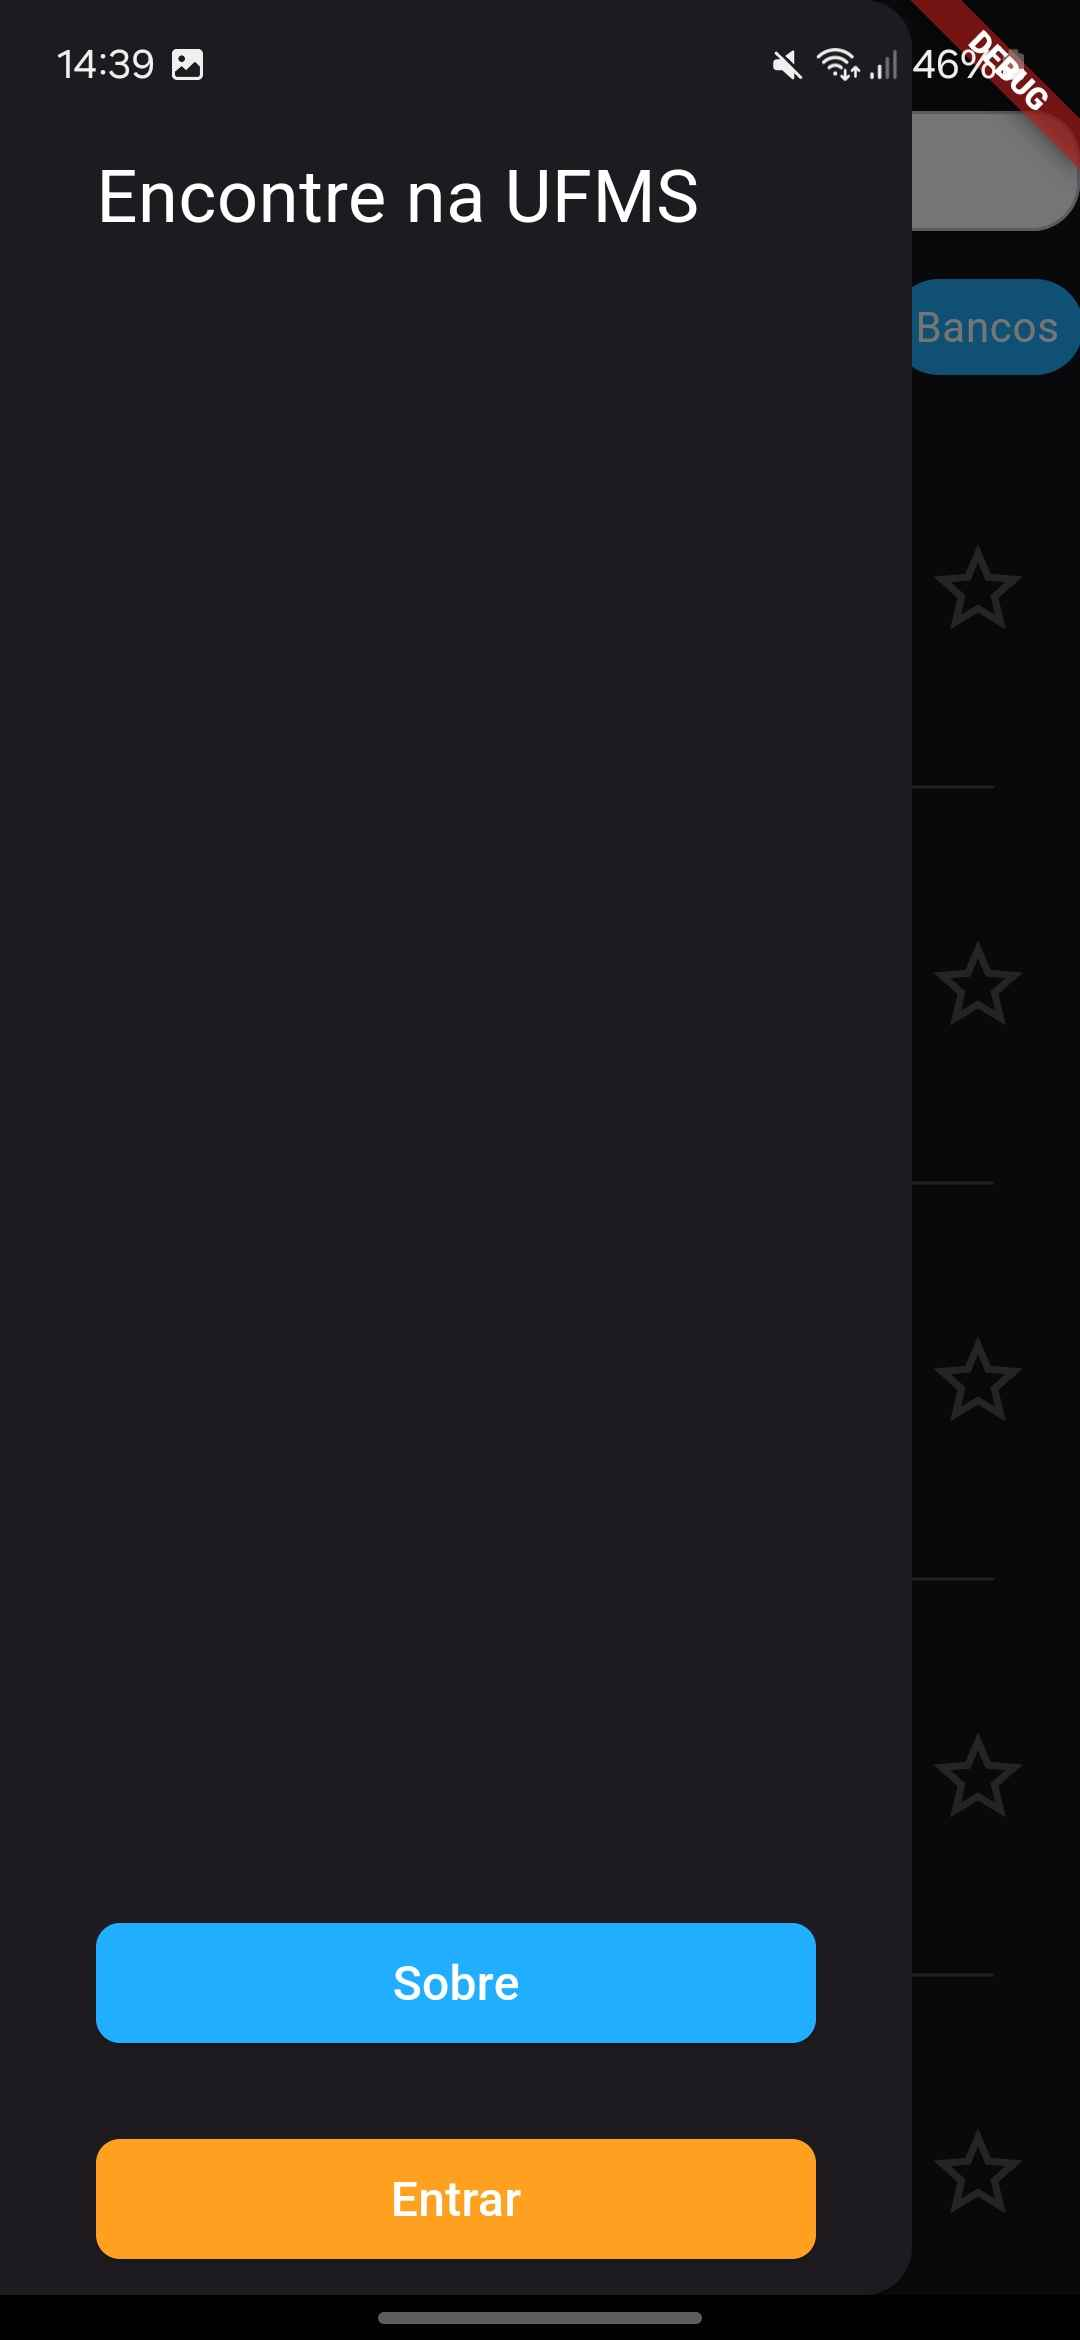
\includegraphics[width=44mm,height=80mm]{imagens/menu-lateral-logout.jpg}
        \caption{\scriptsize Tela 2: Menu Lateral (Logado e Deslogado)}
        \footnotesize  \centering{\textbf{Fonte: Autor original}}
        \label{fig:tela2-logado}
    \end{figure}

    \FloatBarrier

\subsubsection{Tela 4: Perfil}

    A tela de perfil exibe as informações do usuário logado, nome e e-mail. Além disso, a tela também permite que o usuário edite seu nome e altere sua senha. A tela de perfil é uma forma de o usuário gerenciar suas informações pessoais e garantir que seus dados estejam sempre atualizados.

    \begin{figure}[h]
        \centering
        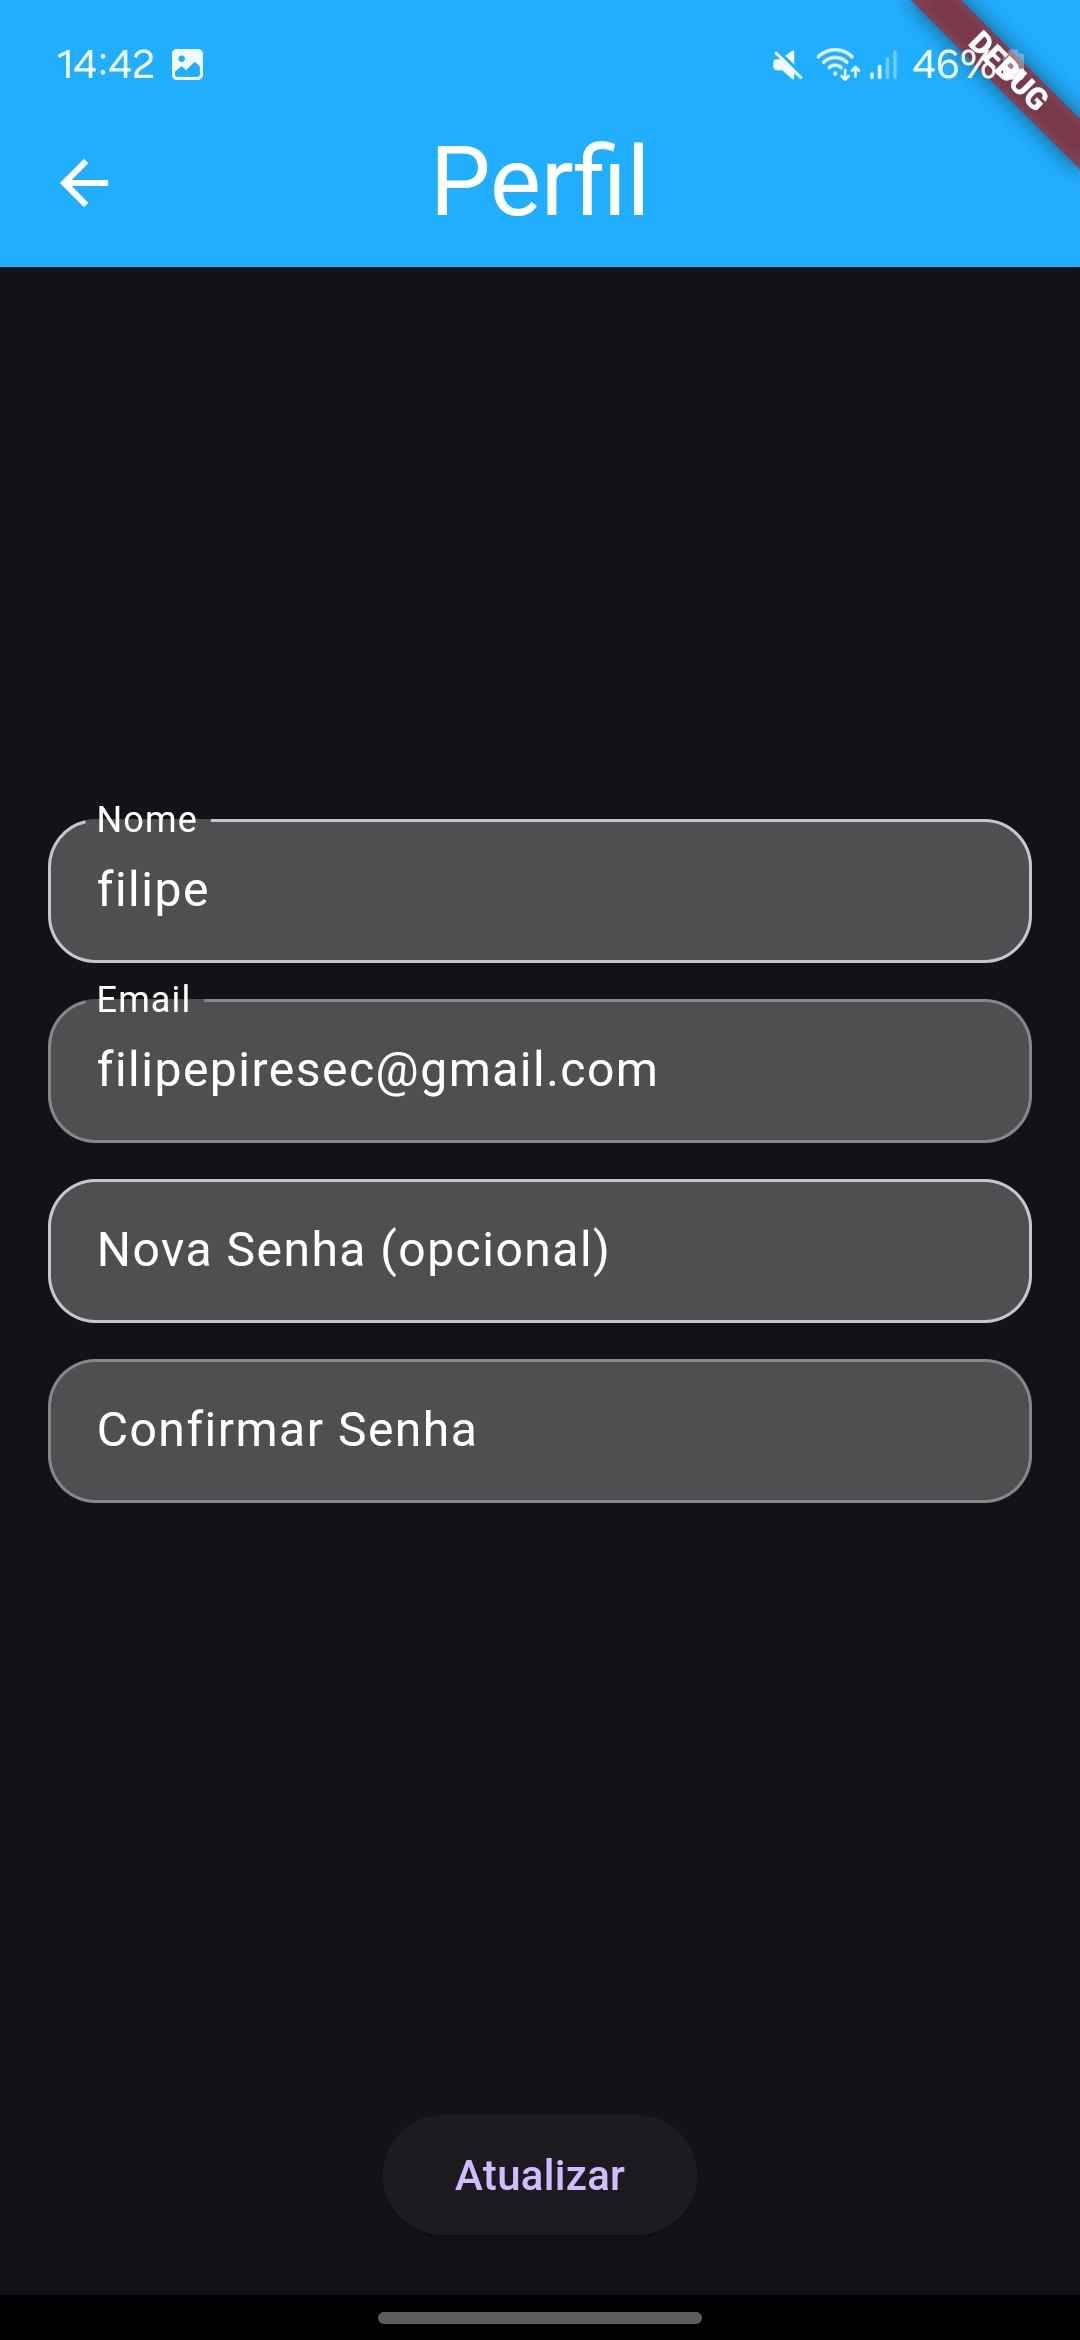
\includegraphics[width=44mm,height=80mm]{imagens/perfil.jpg}
        \caption{\scriptsize Tela 4: Perfil}
        \footnotesize  \centering{\textbf{Fonte: Autor original}}
        \label{fig:tela4}
    \end{figure}

    \FloatBarrier

\subsubsection{Tela 5: Criação}

    A tela de criação possibilita que os usuários preencham uma série de informações sobre o local que desejam cadastrar, como nome, endereço, categoria, horários de funcionamento, telefone de contato, observações e fotos, e enviem para uma avaliação. A tela de criação é uma forma de os usuários contribuírem com o aplicativo, adicionando novos locais e enriquecendo a base de dados do sistema.

    \begin{figure}[h]
        \centering
        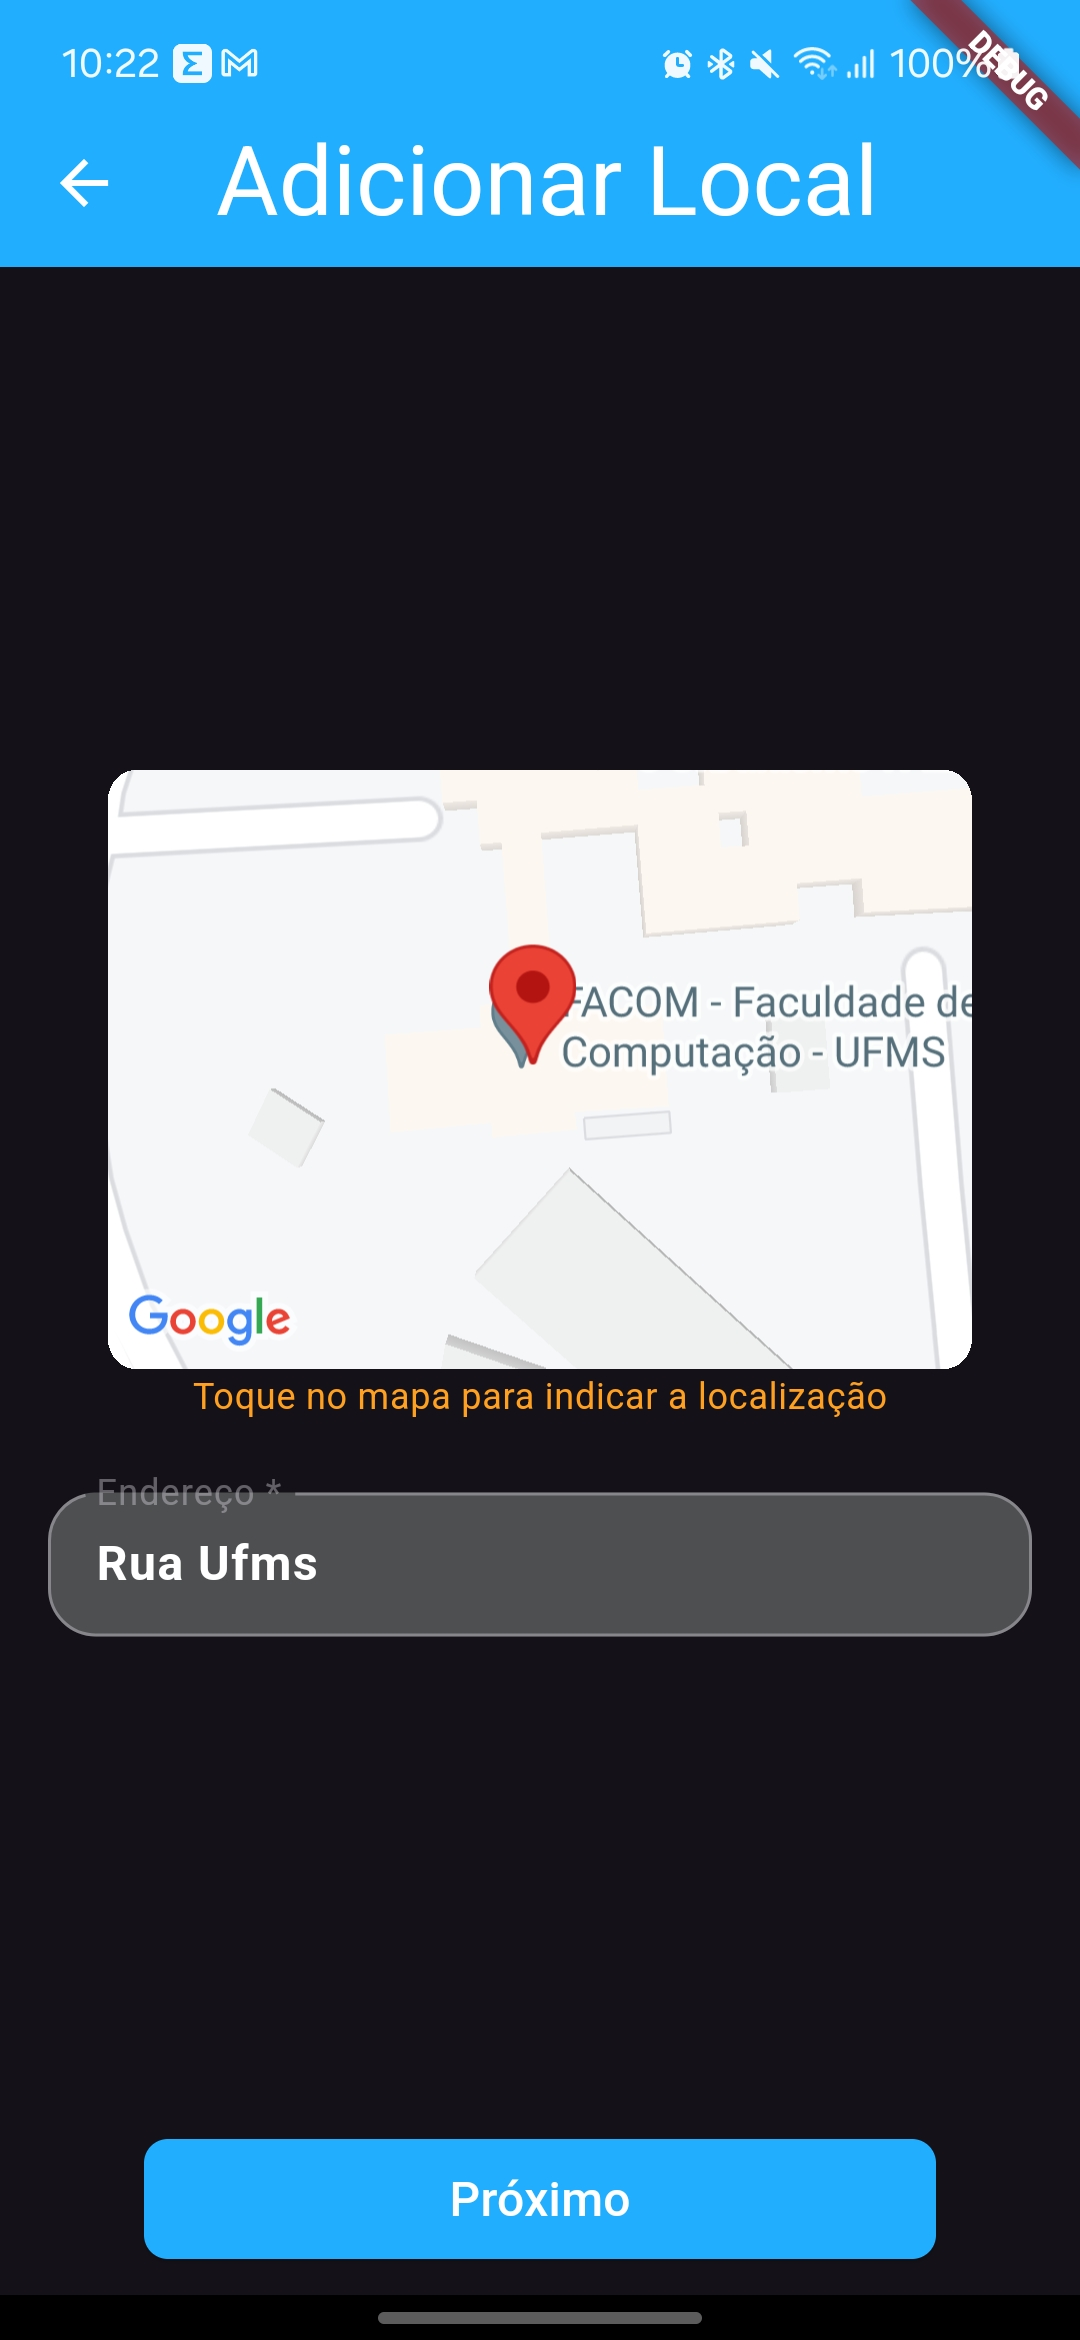
\includegraphics[width=44mm,height=80mm]{imagens/criacao.jpg}
        \caption{\scriptsize Tela 5: Criação}
        \footnotesize  \centering{\textbf{Fonte: Autor original}}
        \label{fig:tela5}
    \end{figure}

    \FloatBarrier

\subsubsection{Tela 6: Sobre}

    A tela de sobre exibe informações sobre o aplicativo, como a versão, os desenvolvedores e a licença de uso. A tela de sobre é uma forma de os usuários conhecerem mais sobre o aplicativo e os desenvolvedores por trás dele.

    \begin{figure}[h]
        \centering
        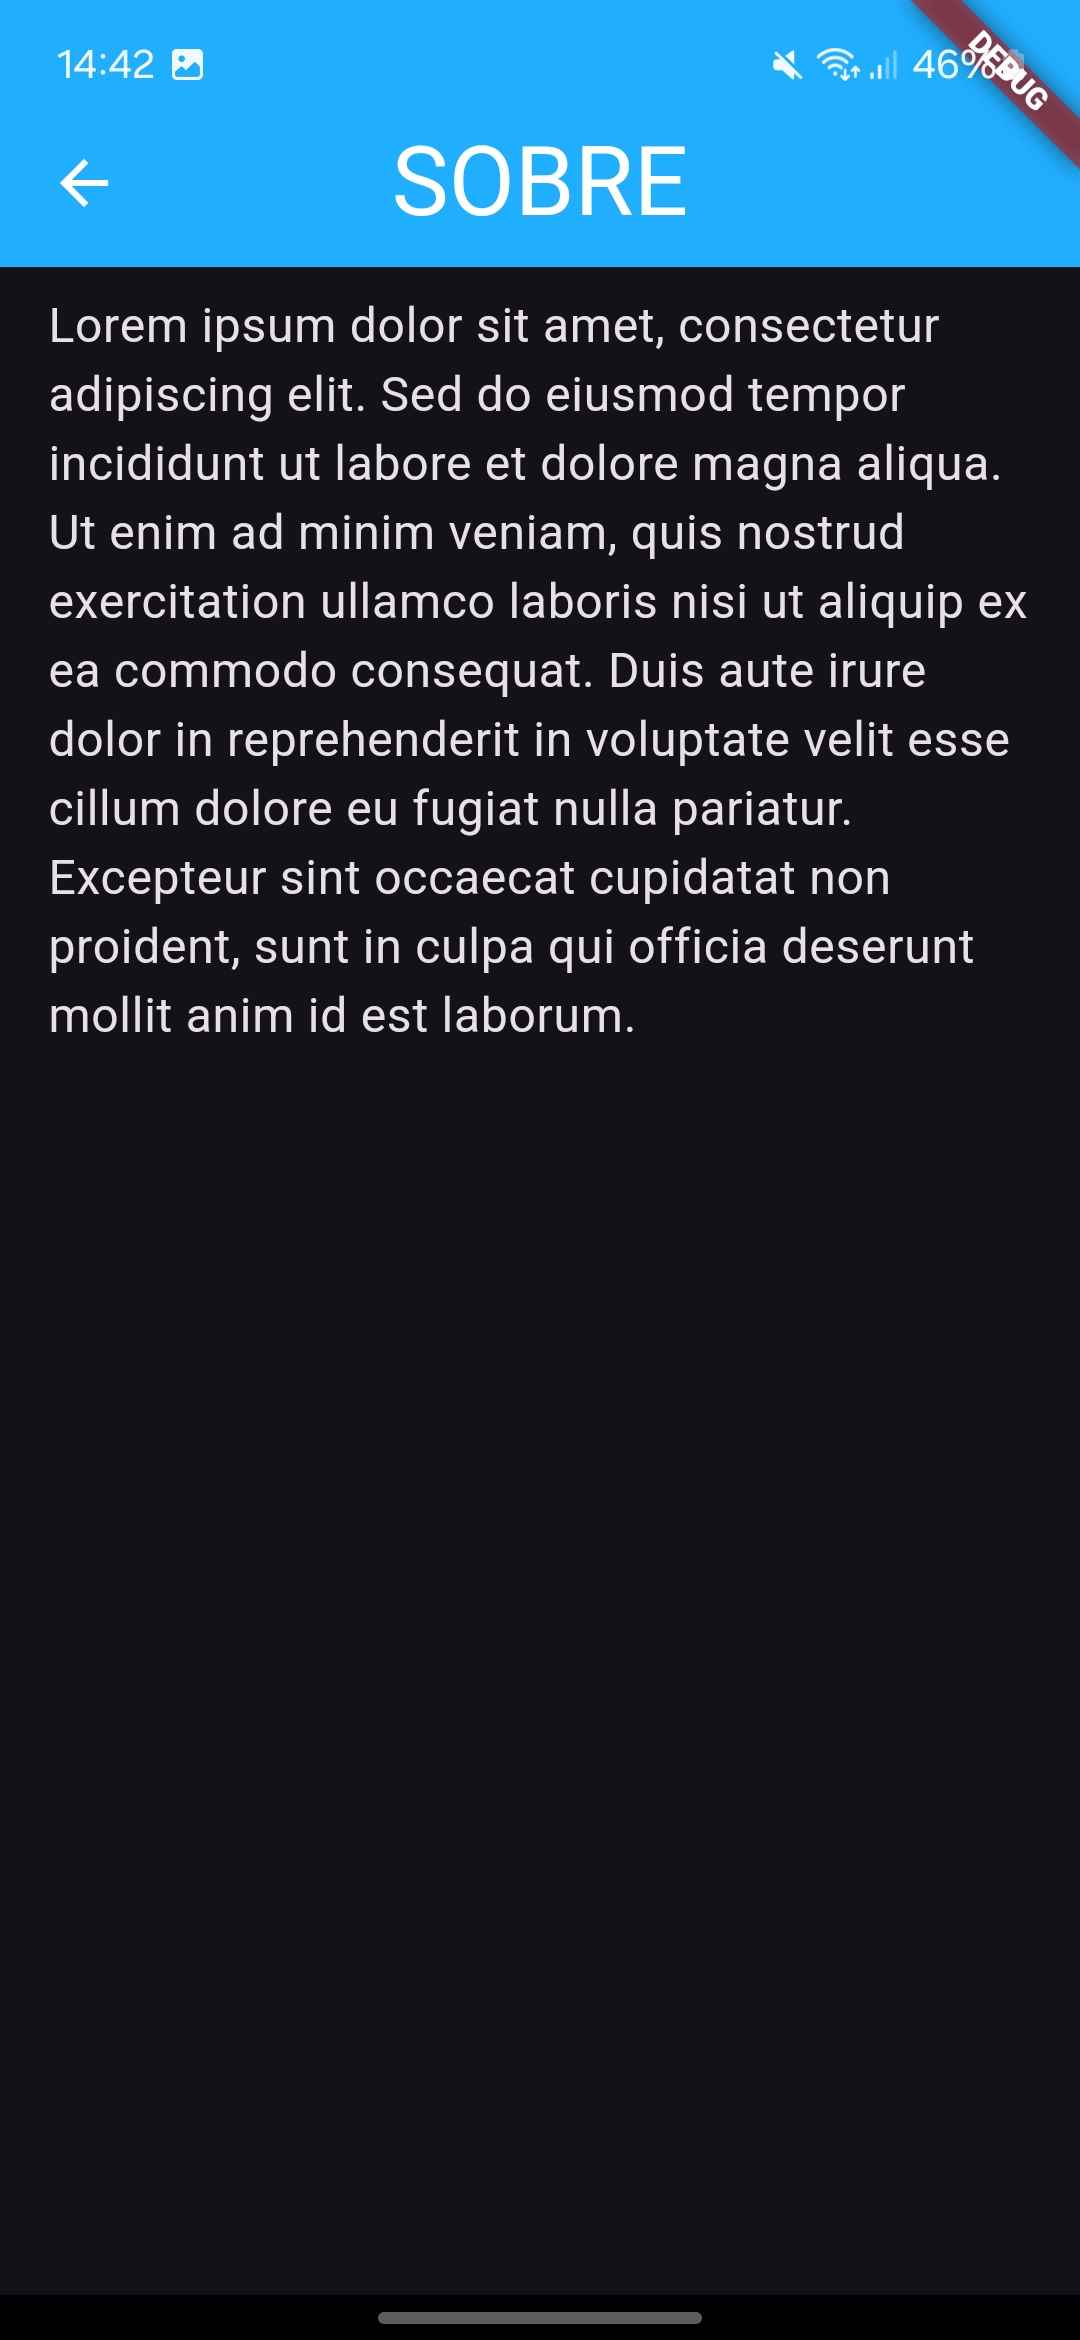
\includegraphics[width=44mm,height=80mm]{imagens/sobre.jpg}
        \caption{\scriptsize Tela 6: Sobre}
        \footnotesize  \centering{\textbf{Fonte: Autor original}}
        \label{fig:tela6}
    \end{figure}

    \FloatBarrier

\subsubsection{Tela 7: Login}

    A tela de login pode ser alcançada através de 2 fluxos, o primeiro é através do botão de Login na tela de Menu Lateral e o segundo é caso o usuário tente marcar um local como favorito sem estar logado. A tela de login é composta por um campo de e-mail e um campo de senha, além de botões para iniciar o processo de registro de uma nova conta ou para recuperar a senha caso o usuário tenha esquecido.

    \begin{figure}[h]
        \centering
        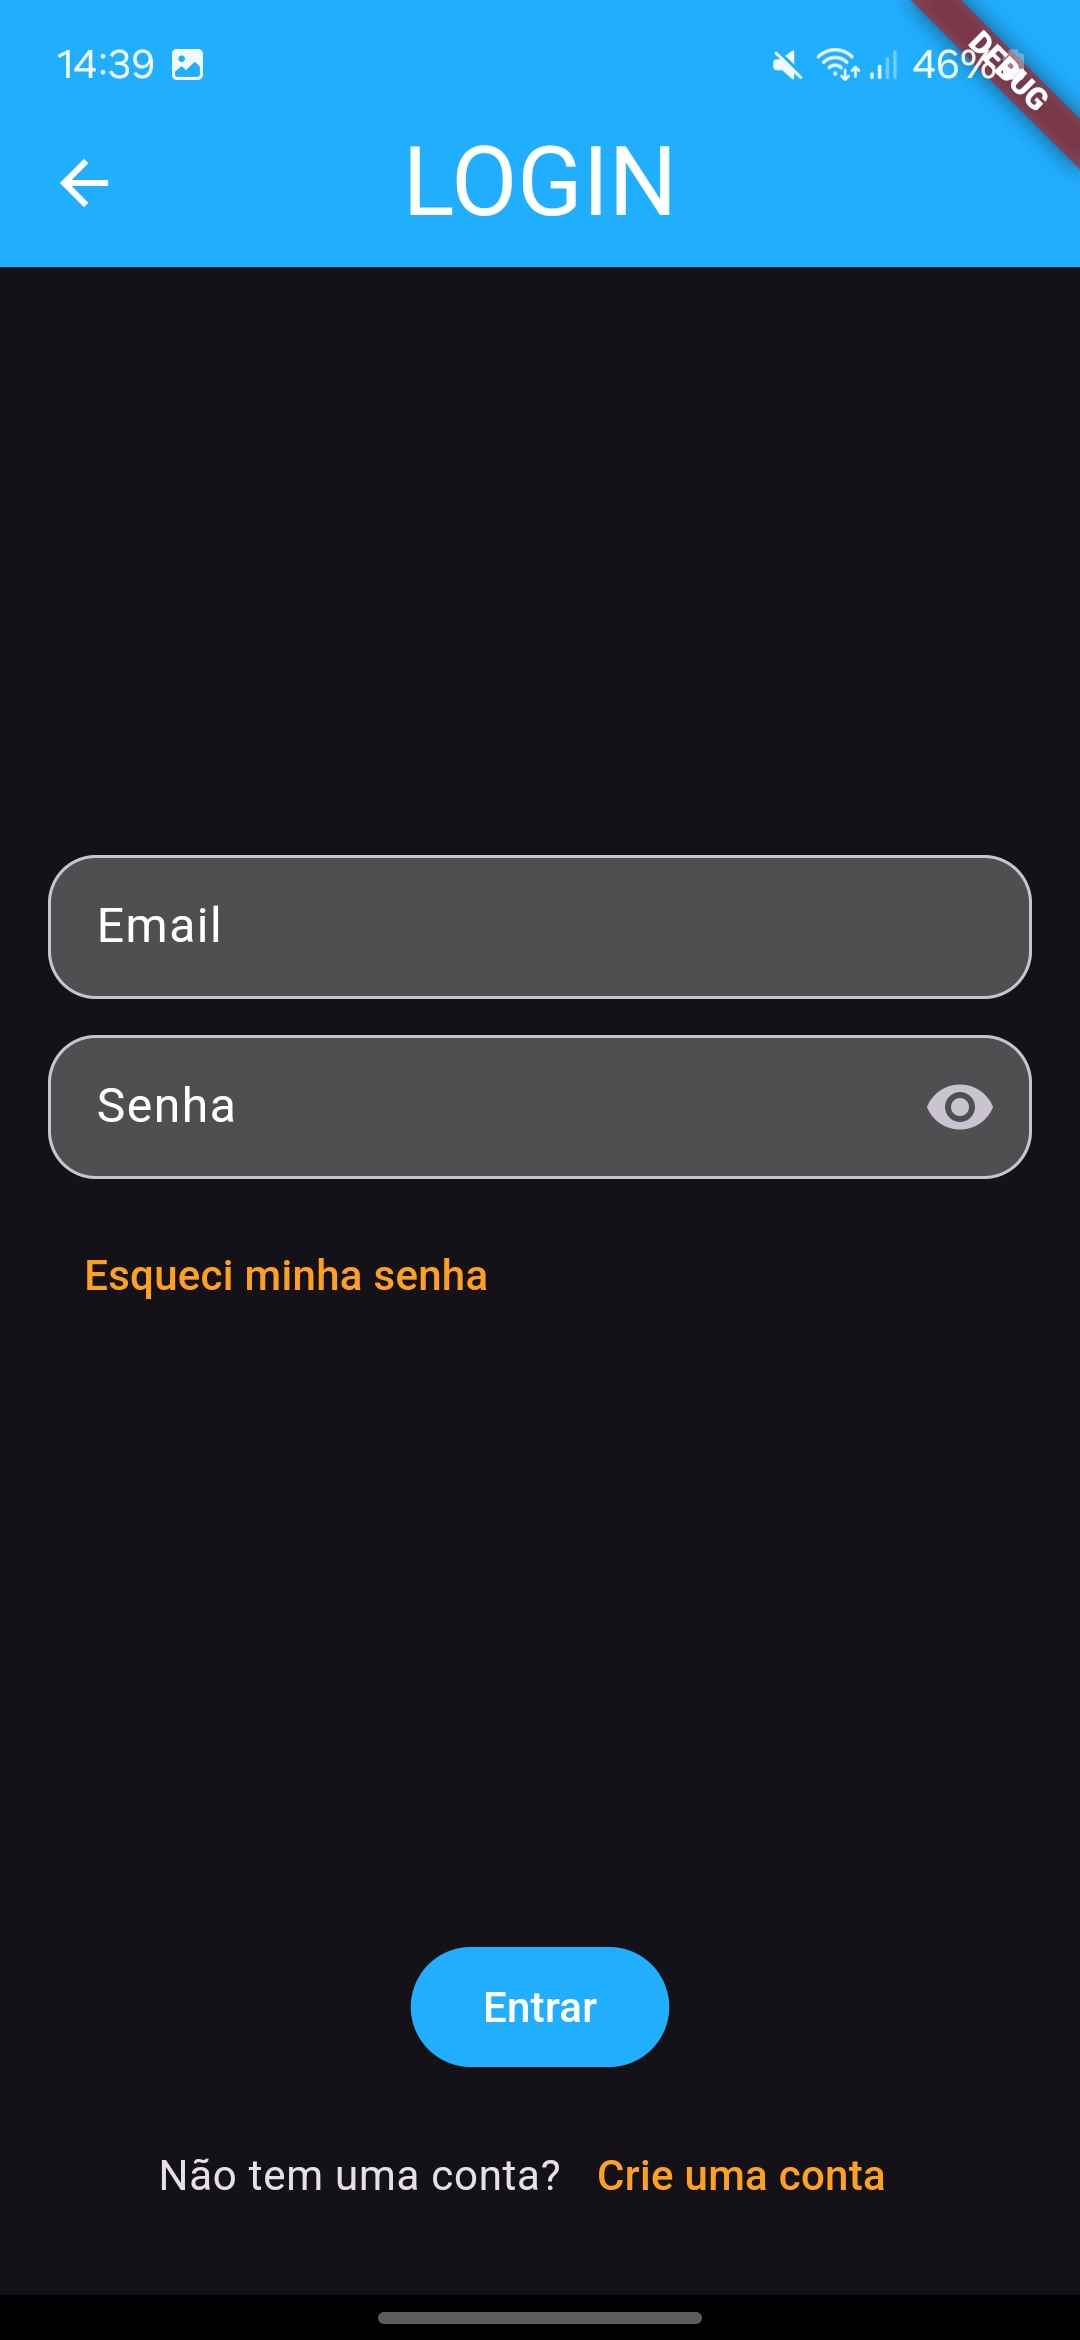
\includegraphics[width=44mm,height=80mm]{imagens/login.jpg}
        \hspace{10mm}
        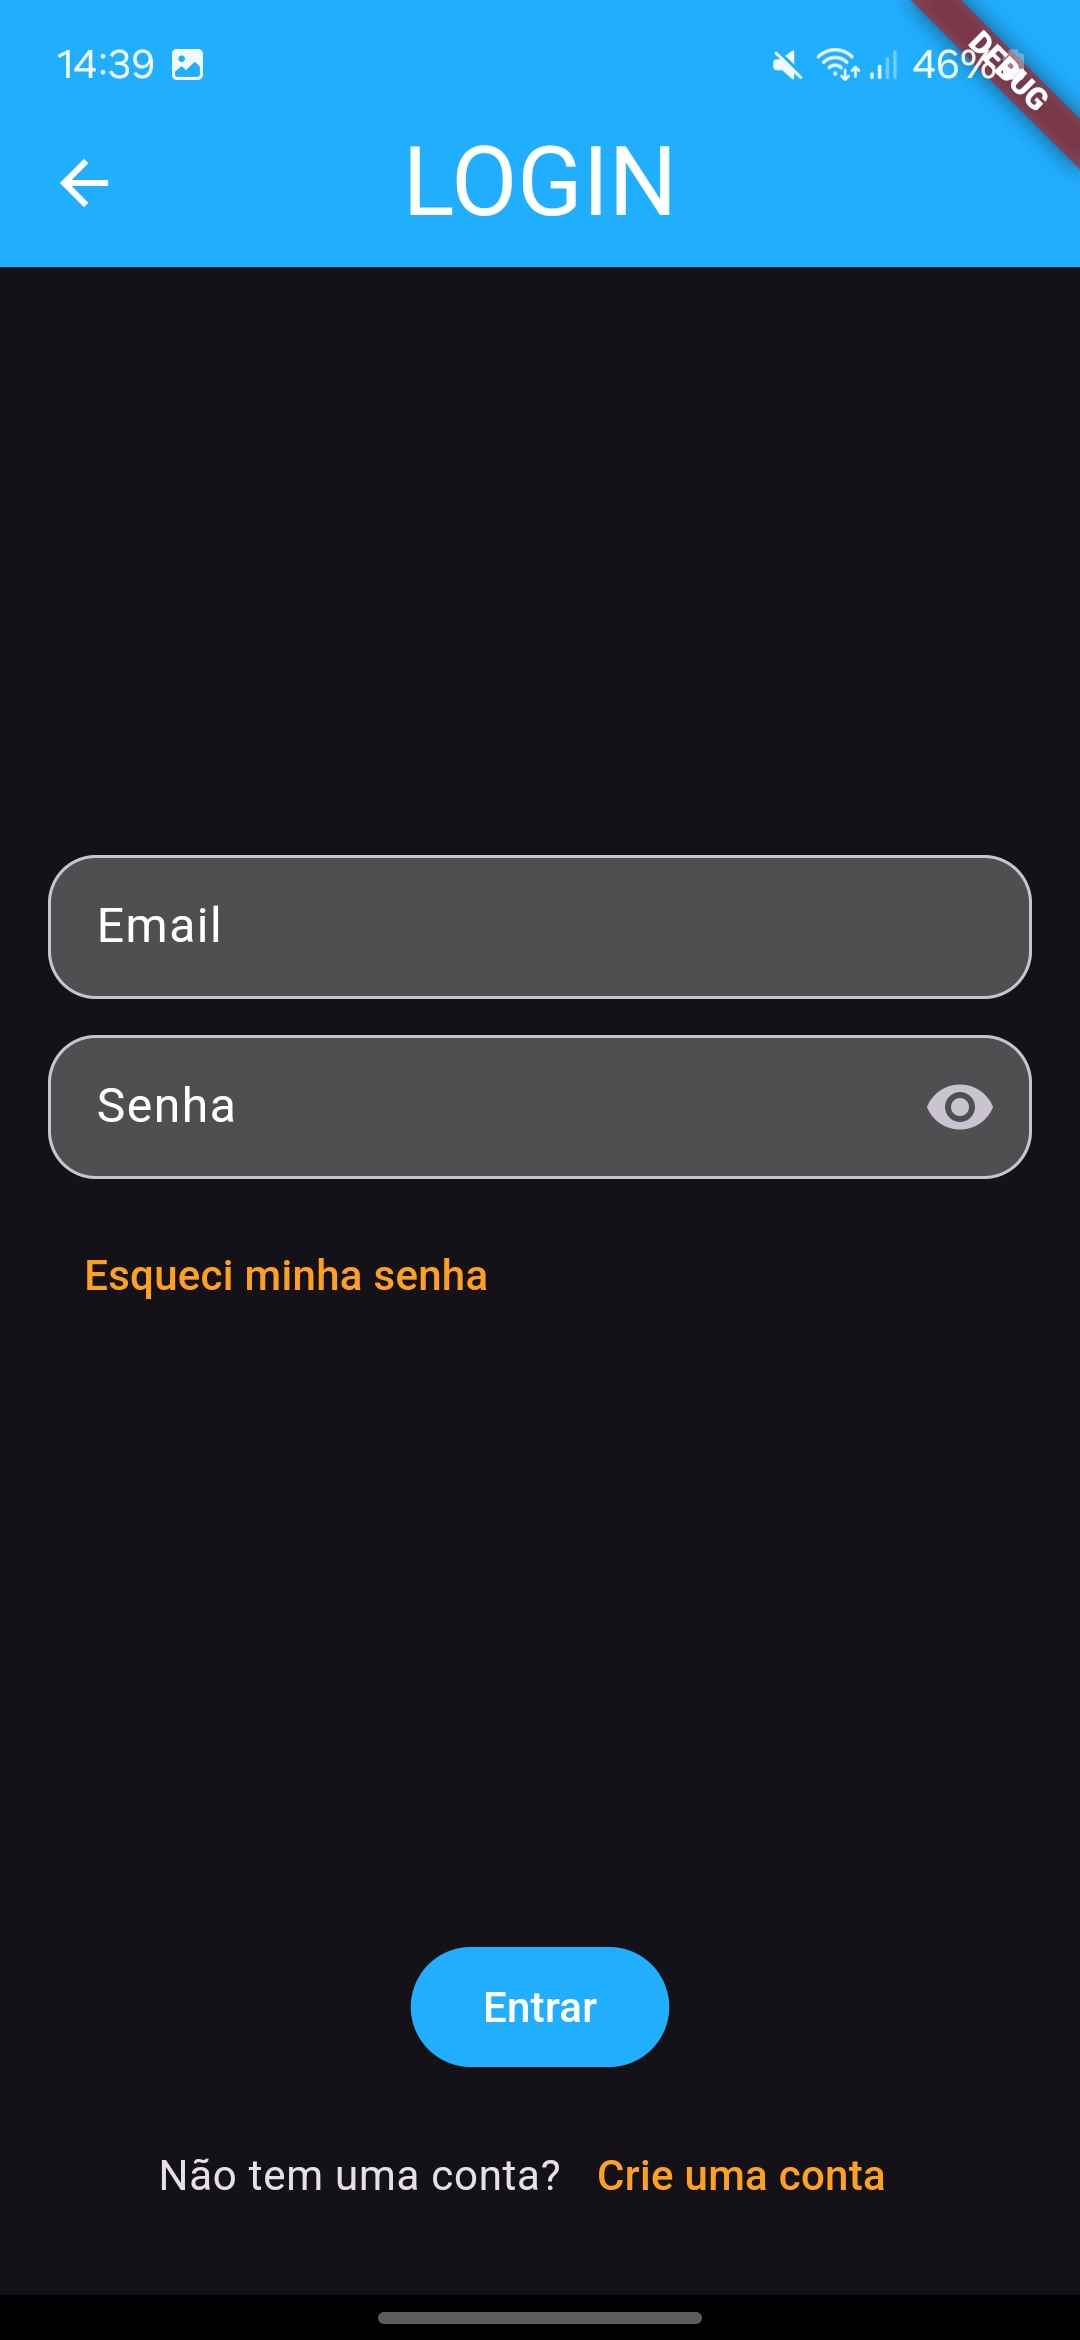
\includegraphics[width=44mm,height=80mm]{imagens/login.jpg} %tela de registro
        \caption{\scriptsize Tela 7: Login}
        \footnotesize  \centering{\textbf{Fonte: Autor original}}
        \label{fig:tela7}
    \end{figure}
    
    Caso o usuário entre no processo de recuperação de senha ele deverá informar o email cadastrado e um email será enviado com um código de recuperação, que deverá ser informado numa tela subsequente, caso a verificação seja bem sucedida o usuário poderá definir uma nova senha.
    
    \FloatBarrier

    \begin{figure}[h]
        \centering
        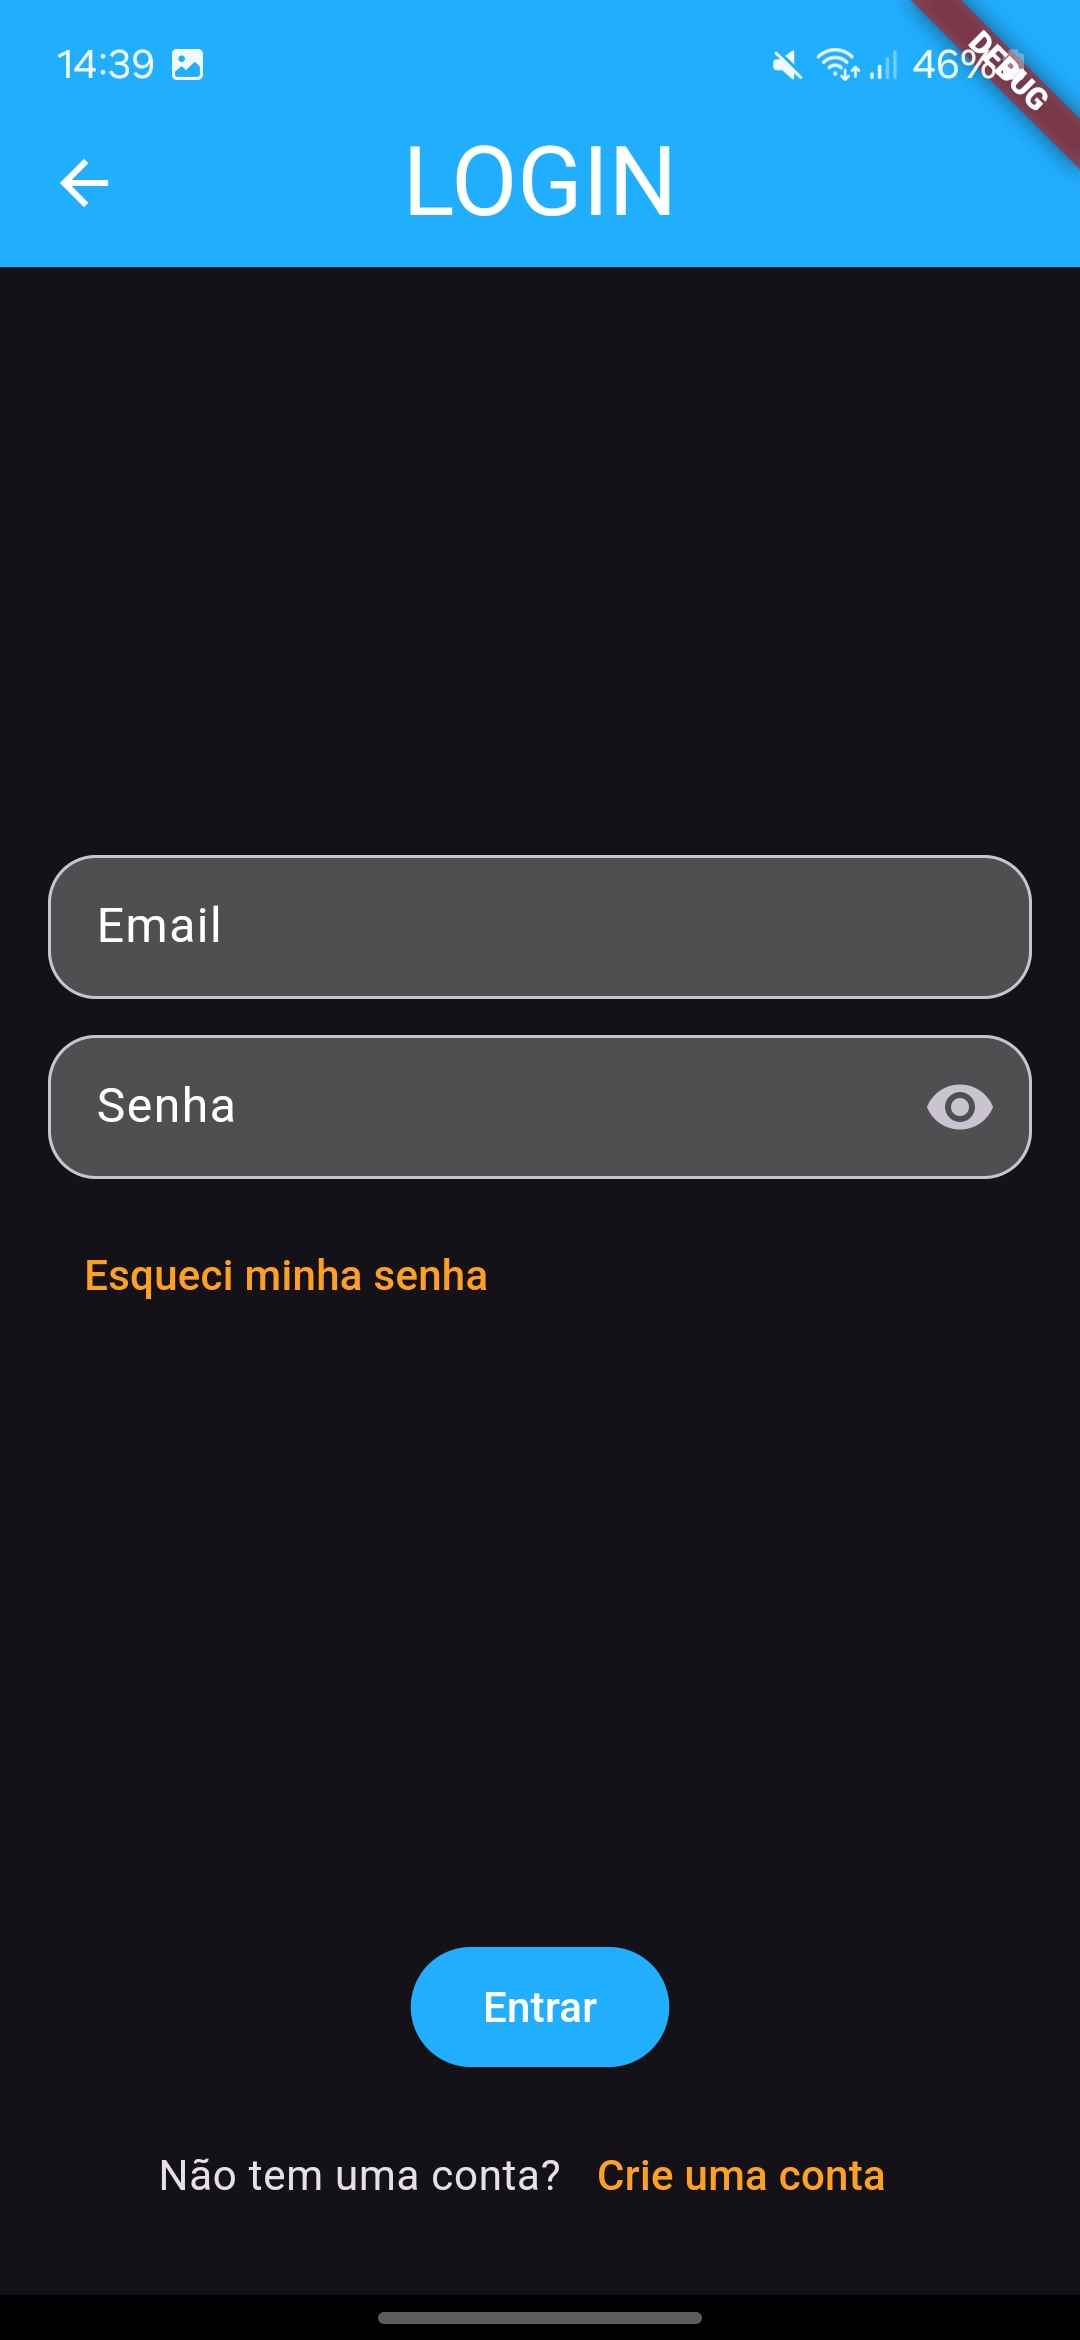
\includegraphics[width=44mm,height=80mm]{imagens/login.jpg} %tela de email
        \hspace{10mm}
        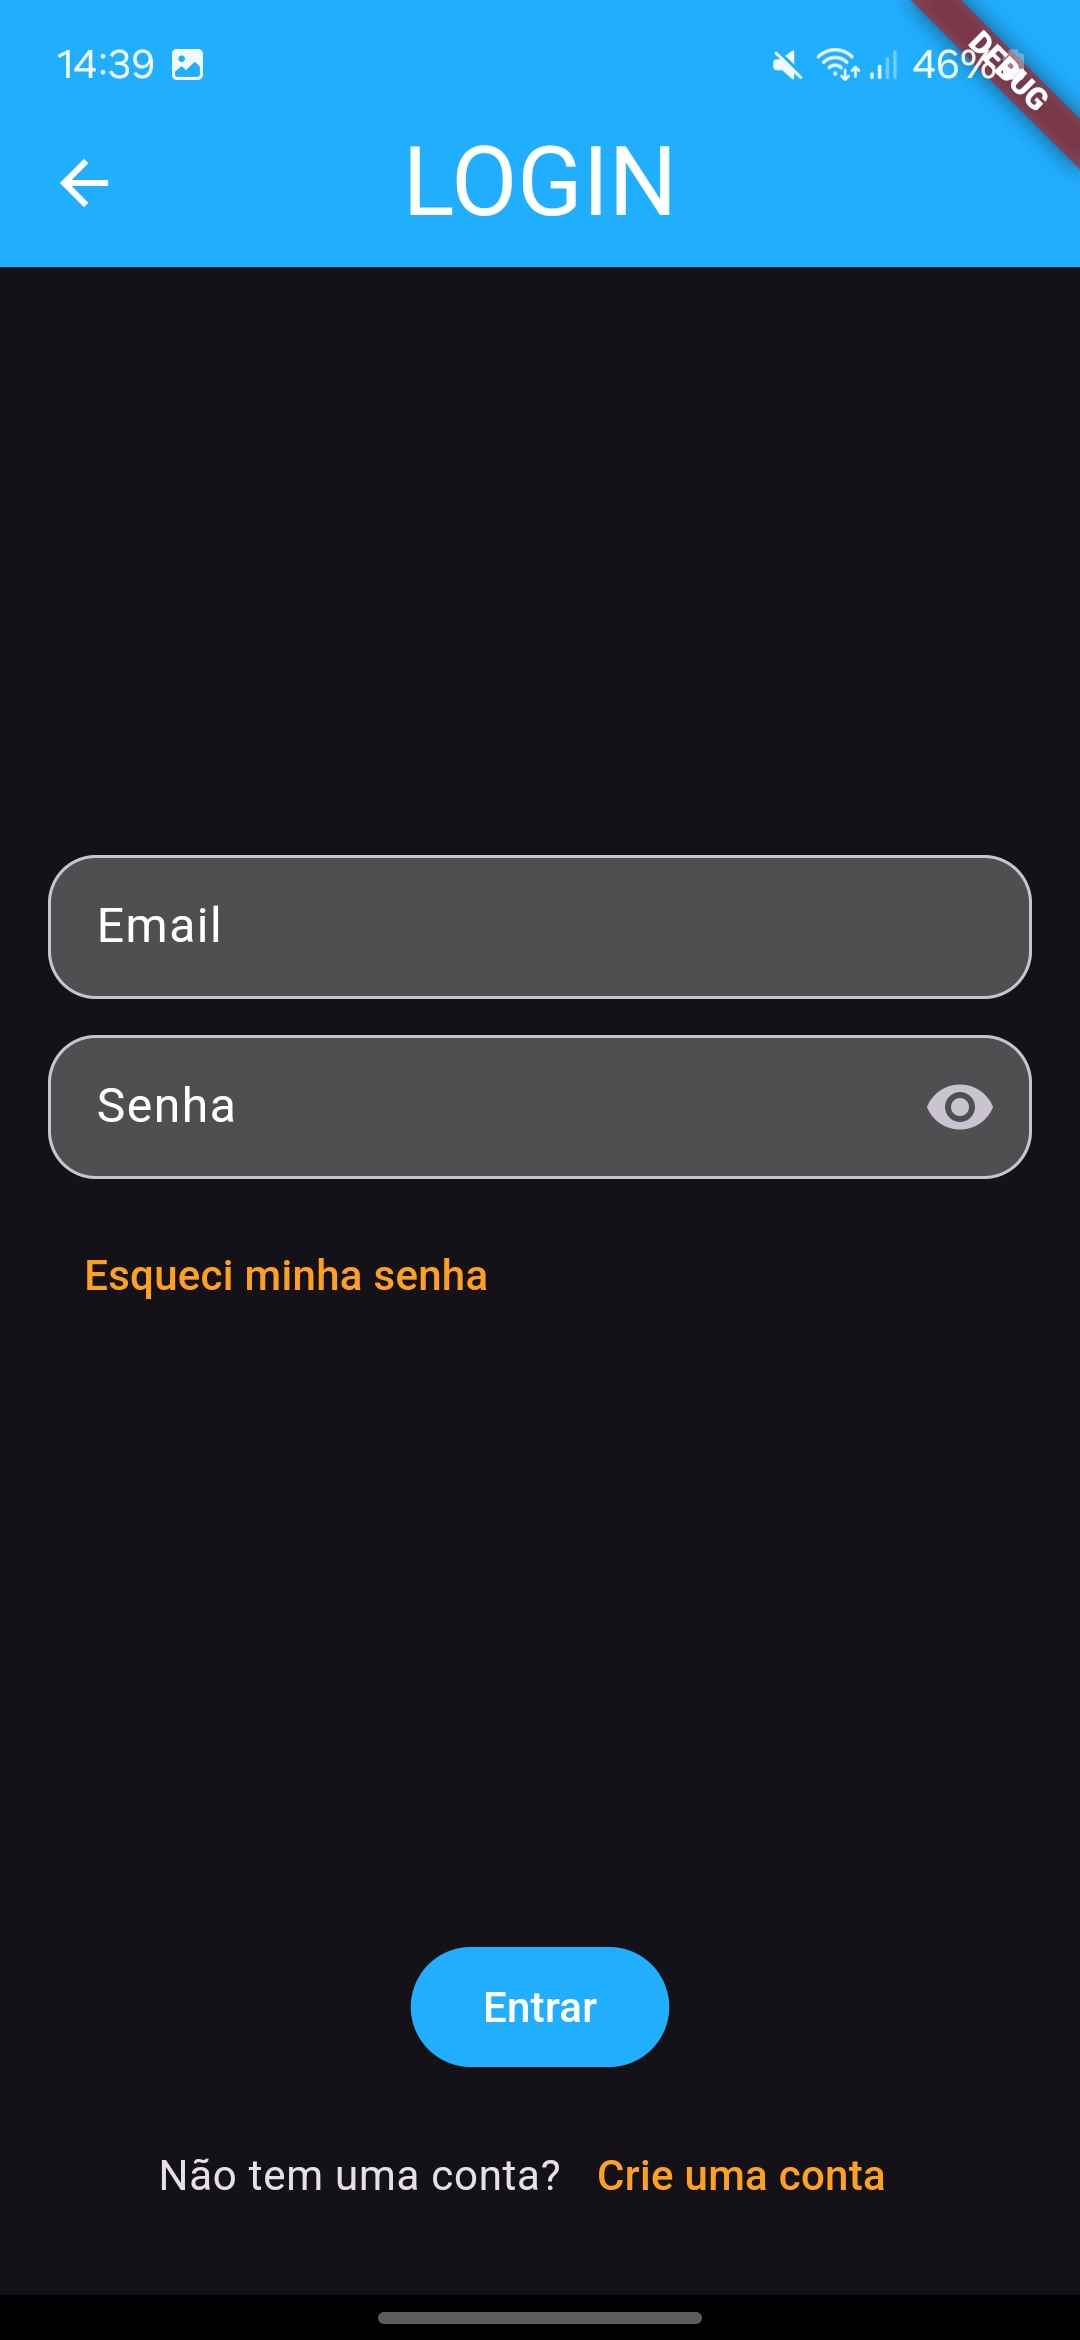
\includegraphics[width=44mm,height=80mm]{imagens/login.jpg} %tela de codigo
        \caption{\scriptsize Tela 7: Login}
        \footnotesize  \centering{\textbf{Fonte: Autor original}}
        \label{fig:tela7-recuperacao}
    \end{figure}

    \FloatBarrier